% !TEX program = xelatex
\documentclass[UTF8,fontset=fandol,a4paper,11pt]{ctexart}
\usepackage[margin=21mm,top=23mm,bottom=22mm,headheight=16pt]{geometry}
\usepackage{amsmath,amssymb,mathtools,bm}
\usepackage{tikz}
\usetikzlibrary{arrows.meta,calc,angles,quotes,patterns}
\usepackage{xcolor,booktabs,array,longtable,enumitem,fancyhdr,needspace}
\usepackage[unicode,hidelinks]{hyperref}
\definecolor{ink}{HTML}{24343C}
\definecolor{accent}{HTML}{166A70}
\definecolor{muted}{HTML}{65747A}
\definecolor{rulegray}{HTML}{D4DDE0}
\definecolor{warm}{HTML}{966037}
\color{ink}
\setlength{\parindent}{2em}
\setlength{\parskip}{4pt}
\linespread{1.12}
\AtBeginDocument{\setlength{\abovedisplayskip}{6pt plus 2pt minus 1pt}
\setlength{\belowdisplayskip}{6pt plus 2pt minus 1pt}
\setlength{\abovedisplayshortskip}{0pt plus 1pt}
\setlength{\belowdisplayshortskip}{4pt plus 1pt}}
\setlist[enumerate]{label=(\arabic*),leftmargin=2.3em,itemsep=3pt,topsep=4pt}
\setlist[itemize]{leftmargin=2em,itemsep=2pt,topsep=4pt}
\allowdisplaybreaks[1]
\setlength{\emergencystretch}{2em}
\setcounter{secnumdepth}{0}
\providecommand{\tightlist}{\setlength{\itemsep}{0pt}\setlength{\parskip}{0pt}}
\ctexset{section={format=\Large\bfseries\color{accent},beforeskip=10pt,afterskip=9pt},
subsection={format=\normalsize\bfseries\color{accent},beforeskip=10pt,afterskip=4pt},
subsubsection={format=\normalsize\bfseries,beforeskip=8pt,afterskip=3pt}}
\pagestyle{fancy}
\fancyhf{}
\fancyhead[L]{\small\color{muted}物理学难题集萃}
% 页眉仅保留书名；版本名称只在封面显示。
\fancyfoot[L]{\small\color{muted}\chapterlabel}
\fancyfoot[R]{\small\thepage}
\renewcommand{\headrulewidth}{0.4pt}
\renewcommand{\footrulewidth}{0pt}
\newcommand{\dd}{\mathop{}\!\mathrm{d}}
\newcommand{\vect}[1]{\bm{#1}}
\newcommand{\tagline}[1]{\noindent{\small\color{muted}#1}\par}
\newcommand{\result}[1]{\begin{equation*}\boxed{#1}\end{equation*}}
\newcommand{\figcaption}[1]{\par\vspace{2pt}{\small\color{muted}#1}\par}
\newcommand{\teach}[2]{\Needspace{4\baselineskip}\subsection*{讲解要点与追问}#1\par\smallskip\noindent\textbf{追问：}#2\par}
\newcommand{\workarea}{\par\vspace{7mm}\noindent{\small\color{muted}作答区}\par\vspace{4mm}
\noindent\textcolor{rulegray}{\rule{\linewidth}{0.3pt}}\par\vspace{16mm}
\noindent\textcolor{rulegray}{\rule{\linewidth}{0.3pt}}\par\vspace{16mm}
\noindent\textcolor{rulegray}{\rule{\linewidth}{0.3pt}}\par\vspace{16mm}
\noindent\textcolor{rulegray}{\rule{\linewidth}{0.3pt}}}
\tikzset{axis/.style={-{Stealth[length=2mm]},thin,color=muted},
motion/.style={-{Stealth[length=2.3mm]},thick,color=accent},
force/.style={-{Stealth[length=2.3mm]},thick,color=warm},
traj/.style={thick,color=accent},guide/.style={dashed,thin,color=muted},
object/.style={thick,color=ink},every node/.style={font=\small}}\widowpenalty=10000\clubpenalty=10000\displaywidowpenalty=10000\newcommand{\chapterlabel}{近代物理第一章\quad 量子物理}







\hypersetup{pdftitle={近代物理第一章 量子物理·学生版},pdfauthor={}}

\begin{document}\pdfbookmark[0]{近代物理第一章 量子物理}{cover}

\thispagestyle{empty}\vspace*{22mm}

\noindent{\Huge\bfseries 物理学难题集萃}\par\vspace{10mm}

\noindent{\LARGE 近代物理第一章}\par\vspace{6mm}

\noindent{\LARGE 量子物理}\par\vspace{12mm}

\noindent{\Large\color{accent}学生版}\par\vspace{9mm}

\noindent\textcolor{accent}{\rule{\linewidth}{1pt}}\par\vspace{9mm}

\noindent 第1--20题\par\vfill\clearpage

\pdfbookmark[1]{题目目录}{contents}\section*{题目目录}

\begin{longtable}{@{}r p{113mm} r@{}}\toprule 题号 & 题目 & 页码\\\midrule

\hyperref[q:1]{1} & \hyperref[q:1]{斜入射光压与切向力} & \pageref{q:1} \\

\hyperref[q:2]{2} & \hyperref[q:2]{非均匀激光束中的微棱镜} & \pageref{q:2} \\

\hyperref[q:3]{3} & \hyperref[q:3]{圆偏振光驱动黑球的螺线运动} & \pageref{q:3} \\

\hyperref[q:4]{4} & \hyperref[q:4]{多层黑板间的辐射传热} & \pageref{q:4} \\

\hyperref[q:5]{5} & \hyperref[q:5]{真空包层下液氦的蒸发} & \pageref{q:5} \\

\hyperref[q:6]{6} & \hyperref[q:6]{黑体谱峰的温度标度} & \pageref{q:6} \\

\hyperref[q:7]{7} & \hyperref[q:7]{太阳照射下的卫星热平衡} & \pageref{q:7} \\

\hyperref[q:8]{8} & \hyperref[q:8]{由光电子磁轨道求逸出功} & \pageref{q:8} \\

\hyperref[q:9]{9} & \hyperref[q:9]{自由电子为何不能完整吸收单光子} & \pageref{q:9} \\

\hyperref[q:10]{10} & \hyperref[q:10]{已知散射波长的康普顿反冲} & \pageref{q:10} \\

\hyperref[q:11]{11} & \hyperref[q:11]{由电子反冲方向求能量} & \pageref{q:11} \\

\hyperref[q:12]{12} & \hyperref[q:12]{最大能量转移反求入射波长} & \pageref{q:12} \\

\hyperref[q:13]{13} & \hyperref[q:13]{光子与电子散射角的关系} & \pageref{q:13} \\

\hyperref[q:14]{14} & \hyperref[q:14]{氢氘谱线与核质量比} & \pageref{q:14} \\

\hyperref[q:15]{15} & \hyperref[q:15]{缪子类氢离子的半径与结合能} & \pageref{q:15} \\

\hyperref[q:16]{16} & \hyperref[q:16]{多普勒光谱测离子速度分布} & \pageref{q:16} \\

\hyperref[q:17]{17} & \hyperref[q:17]{钠原子束的激光减速} & \pageref{q:17} \\

\hyperref[q:18]{18} & \hyperref[q:18]{两次逆向康普顿过程与电子物质波} & \pageref{q:18} \\

\hyperref[q:19]{19} & \hyperref[q:19]{带电细丝的电子双棱镜} & \pageref{q:19} \\

\hyperref[q:20]{20} & \hyperref[q:20]{气体复合的不确定尺度模型} & \pageref{q:20} \\

\bottomrule\end{longtable}

\clearpage

\pdfbookmark[2]{第 1 题 斜入射光压与切向力}{q1}

\section*{第 1 题\quad 斜入射光压与切向力}\label{q:1}

光束以入射角$i$照到不透明的平面上，光束垂直截面的能流密度为$I$，表面的能量反射率为$R$。反射为镜面反射，其余入射光被吸收。求单位实际表面积受到的法向光压和切向力；忽略受热后的再辐射。

\begin{center}\begin{minipage}{.98\linewidth}\centering
\begin{tikzpicture}[scale=.9,transform shape]
\draw[object] (-3.00000,0.00000)--(3.00000,0.00000);\fill (0.00000,0.00000) circle(.035);\node[below left] at (0.00000,0.00000) {$O$};\draw[motion] (-2.00000,2.00000)--(0.00000,0.00000);
\draw[motion] (0.00000,0.00000)--(2.00000,2.00000);\draw[axis] (0.00000,0.00000)--(0.00000,-1.70000);\draw[axis] (0.00000,0.00000)--(3.00000,0.00000);\node[below] at (0.00000,-1.70000) {$\hat n$};\node[below right] at (3.00000,0.00000) {$\hat t$};\node[above] at (-0.40000,1.00000) {$i$};\node[above] at (2.00000,-1.15000) {实际表面 $\dd S$};\node[above] at (-2.30000,2.00000) {$I,\dd S_\perp$};
\end{tikzpicture}
\figcaption{图近1.1\quad 入射、镜面反射与两种面积定义。}
\end{minipage}\end{center}

\workarea

\clearpage

\pdfbookmark[2]{第 2 题 非均匀激光束中的微棱镜}{q2}

\section*{第 2 题\quad 非均匀激光束中的微棱镜}\label{q:2}

很小的等腰玻璃三棱镜顶角为$A=\pi-2\alpha$，竖直底边长$2h$，沿$z$的厚度为$w$，折射率$n$、密度$\rho$。顶点朝向从左沿$+x$传播的激光，三角形端面平行$xy$，底面平行$yz$，保持取向不转动；各面理想减反射。激光沿$z$均匀，沿$y$有
\[
I(y)=I_0\left(1-\frac{|y|}{4h}\right)\quad(|y|\leqslant4h),
\]
其他位置为零。棱镜尖端位于$y=y_0$，$|y_0|\leqslant3h$，忽略光强随$x$改变和运动的多普勒修正。
\begin{enumerate}[label=（\arabic*）]
\item 求进入上斜面、由竖直底面射出光线的向下偏转角$\theta$。
\item 计算光给棱镜的$F_x,F_y$，并画随$y_0$变化的曲线。
\item 取$\alpha=30^\circ,h=10\,\mu\mathrm m,n=1.5,w=1\,\mathrm{mm},\rho=2.5\times10^3\,\mathrm{kg/m^3}$。激光全宽为$80\,\mu\mathrm m$、$z$宽1mm，棱镜在$y_0=-h/2$，求使竖直光力平衡重力所需的光束总功率。取$g=9.8\,\mathrm{m/s^2},c=3.00\times10^8\,\mathrm{m/s}$，说明水平方向的条件。
\item 无重力时，取$I_0=10^8\,\mathrm{W/m^2}$，从$y_0=h/20$静止释放，求竖直小振动周期。水平光力另由约束平衡。
\end{enumerate}

\begin{center}\begin{minipage}{.98\linewidth}\centering
\begin{tikzpicture}[scale=.9,transform shape]
\draw[object] (0.00000,0.00000)--(0.98150,1.70000)--(0.98150,-1.70000)--(0.00000,0.00000);\draw[<->,thin,color=muted] (1.48150,-1.70000)--(1.48150,1.70000);\node[right] at (1.48150,0.00000) {$2h$};\node[left] at (-0.10000,0.20000) {$A$};\draw[motion] (-2.20000,-1.00000)--(0.57735,-1.00000);\draw[motion] (-2.20000,-0.50000)--(0.28868,-0.50000);\draw[motion] (-2.20000,0.50000)--(0.28868,0.50000);\draw[motion] (-2.20000,1.00000)--(0.57735,1.00000);\node[above] at (0.98150,2.05000) {$\alpha$};\node[below] at (0.00000,-2.20000) {$+x$ 向右，$y_0$为顶点高度};
\end{tikzpicture}
\figcaption{图近1.2\quad 固定取向的微棱镜及上下入射光束。}
\end{minipage}\end{center}

\workarea

\clearpage

\pdfbookmark[2]{第 3 题 圆偏振光驱动黑球的螺线运动}{q3}

\section*{第 3 题\quad 圆偏振光驱动黑球的螺线运动}\label{q:3}

均匀黑色实心球半径$r=1\,\mathrm{mm}$，在无重力空间起初静止。均匀平行圆偏振激光沿一条直径方向照遍球的迎光截面，真空波长$\lambda=10^4\,\mathrm{nm}$。每个被吸收光子具有能量$h\nu$、动量$h/\lambda$和沿传播轴或反向的自旋角动量$\pm\hbar$。讨论时间内激光强度保持不变。忽略吸收导致的质量改变、热辐射和高速修正，求球上轴外各点轨迹的螺距。

\begin{center}\begin{minipage}{.98\linewidth}\centering
\begin{tikzpicture}[scale=.9,transform shape]
\draw[object] (2.00000,0.00000) circle(1.20000);\draw[axis] (-2.00000,0.00000)--(2.00000,0.00000);
\draw[axis] (2.00000,0.00000)--(4.00000,0.00000);\node[below right] at (4.00000,0.00000) {$x$};\draw[traj] plot coordinates {(-2.00000,-0.80000) (-1.97842,-0.78568) (-1.95683,-0.77286) (-1.93525,-0.76285) (-1.91367,-0.75670) (-1.89209,-0.75505) (-1.87050,-0.75807) (-1.84892,-0.76545) (-1.82734,-0.77642) (-1.80576,-0.78983) (-1.78417,-0.80431) (-1.76259,-0.81833) (-1.74101,-0.83045) (-1.71942,-0.83941) (-1.69784,-0.84427) (-1.67626,-0.84454) (-1.65468,-0.84017) (-1.63309,-0.83163) (-1.61151,-0.81981) (-1.58993,-0.80593) (-1.56835,-0.79143) (-1.54676,-0.77782) (-1.52518,-0.76652) (-1.50360,-0.75869) (-1.48201,-0.75516) (-1.46043,-0.75628) (-1.43885,-0.76195) (-1.41727,-0.77157) (-1.39568,-0.78415) (-1.37410,-0.79837) (-1.35252,-0.81276) (-1.33094,-0.82582) (-1.30935,-0.83621) (-1.28777,-0.84283) (-1.26619,-0.84500) (-1.24460,-0.84249) (-1.22302,-0.83557) (-1.20144,-0.82496) (-1.17986,-0.81175) (-1.15827,-0.79732) (-1.13669,-0.78317) (-1.11511,-0.77077) (-1.09353,-0.76140) (-1.07194,-0.75605) (-1.05036,-0.75526) (-1.02878,-0.75912) (-1.00719,-0.76723) (-0.98561,-0.77874) (-0.96403,-0.79246) (-0.94245,-0.80696) (-0.92086,-0.82074) (-0.89928,-0.83237) (-0.87770,-0.84063) (-0.85612,-0.84467) (-0.83453,-0.84407) (-0.81295,-0.83889) (-0.79137,-0.82967) (-0.76978,-0.81737) (-0.74820,-0.80326) (-0.72662,-0.78882) (-0.70504,-0.77553) (-0.68345,-0.76479) (-0.66187,-0.75770) (-0.64029,-0.75501) (-0.61871,-0.75700) (-0.59712,-0.76345) (-0.57554,-0.77370) (-0.55396,-0.78668) (-0.53237,-0.80105) (-0.51079,-0.81530) (-0.48921,-0.82797) (-0.46763,-0.83773) (-0.44604,-0.84357) (-0.42446,-0.84489) (-0.40288,-0.84154) (-0.38129,-0.83387) (-0.35971,-0.82269) (-0.33813,-0.80915) (-0.31655,-0.79466) (-0.29496,-0.78072) (-0.27338,-0.76879) (-0.25180,-0.76010) (-0.23022,-0.75555) (-0.20863,-0.75563) (-0.18705,-0.76031) (-0.16547,-0.76912) (-0.14388,-0.78113) (-0.12230,-0.79511) (-0.10072,-0.80960) (-0.07914,-0.82308) (-0.05755,-0.83417) (-0.03597,-0.84171) (-0.01439,-0.84492) (0.00719,-0.84346) (0.02878,-0.83748) (0.05036,-0.82761) (0.07194,-0.81487) (0.09353,-0.80059) (0.11511,-0.78624) (0.13669,-0.77333) (0.15827,-0.76318) (0.17986,-0.75686) (0.20144,-0.75503) (0.22302,-0.75786) (0.24460,-0.76508) (0.26619,-0.77592) (0.28777,-0.78926) (0.30935,-0.80372) (0.33094,-0.81779) (0.35252,-0.83002) (0.37410,-0.83912) (0.39568,-0.84416) (0.41727,-0.84462) (0.43885,-0.84043) (0.46043,-0.83205) (0.48201,-0.82034) (0.50360,-0.80651) (0.52518,-0.79201) (0.54676,-0.77833) (0.56835,-0.76691) (0.58993,-0.75893) (0.61151,-0.75521) (0.63309,-0.75615) (0.65468,-0.76164) (0.67626,-0.77112) (0.69784,-0.78360) (0.71942,-0.79778) (0.74101,-0.81219) (0.76259,-0.82534) (0.78417,-0.83585) (0.80576,-0.84264) (0.82734,-0.84500) (0.84892,-0.84268) (0.87050,-0.83593) (0.89209,-0.82545) (0.91367,-0.81232) (0.93525,-0.79791) (0.95683,-0.78372) (0.97842,-0.77122) (1.00000,-0.76171)};\draw[motion] (0.82000,-0.80000)--(1.00000,-0.80000);\draw[traj] plot coordinates {(-2.00000,0.00000) (-1.97842,0.01432) (-1.95683,0.02714) (-1.93525,0.03715) (-1.91367,0.04330) (-1.89209,0.04495) (-1.87050,0.04193) (-1.84892,0.03455) (-1.82734,0.02358) (-1.80576,0.01017) (-1.78417,-0.00431) (-1.76259,-0.01833) (-1.74101,-0.03045) (-1.71942,-0.03941) (-1.69784,-0.04427) (-1.67626,-0.04454) (-1.65468,-0.04017) (-1.63309,-0.03163) (-1.61151,-0.01981) (-1.58993,-0.00593) (-1.56835,0.00857) (-1.54676,0.02218) (-1.52518,0.03348) (-1.50360,0.04131) (-1.48201,0.04484) (-1.46043,0.04372) (-1.43885,0.03805) (-1.41727,0.02843) (-1.39568,0.01585) (-1.37410,0.00163) (-1.35252,-0.01276) (-1.33094,-0.02582) (-1.30935,-0.03621) (-1.28777,-0.04283) (-1.26619,-0.04500) (-1.24460,-0.04249) (-1.22302,-0.03557) (-1.20144,-0.02496) (-1.17986,-0.01175) (-1.15827,0.00268) (-1.13669,0.01683) (-1.11511,0.02923) (-1.09353,0.03860) (-1.07194,0.04395) (-1.05036,0.04474) (-1.02878,0.04088) (-1.00719,0.03277) (-0.98561,0.02126) (-0.96403,0.00754) (-0.94245,-0.00696) (-0.92086,-0.02074) (-0.89928,-0.03237) (-0.87770,-0.04063) (-0.85612,-0.04467) (-0.83453,-0.04407) (-0.81295,-0.03889) (-0.79137,-0.02967) (-0.76978,-0.01737) (-0.74820,-0.00326) (-0.72662,0.01118) (-0.70504,0.02447) (-0.68345,0.03521) (-0.66187,0.04230) (-0.64029,0.04499) (-0.61871,0.04300) (-0.59712,0.03655) (-0.57554,0.02630) (-0.55396,0.01332) (-0.53237,-0.00105) (-0.51079,-0.01530) (-0.48921,-0.02797) (-0.46763,-0.03773) (-0.44604,-0.04357) (-0.42446,-0.04489) (-0.40288,-0.04154) (-0.38129,-0.03387) (-0.35971,-0.02269) (-0.33813,-0.00915) (-0.31655,0.00534) (-0.29496,0.01928) (-0.27338,0.03121) (-0.25180,0.03990) (-0.23022,0.04445) (-0.20863,0.04437) (-0.18705,0.03969) (-0.16547,0.03088) (-0.14388,0.01887) (-0.12230,0.00489) (-0.10072,-0.00960) (-0.07914,-0.02308) (-0.05755,-0.03417) (-0.03597,-0.04171) (-0.01439,-0.04492) (0.00719,-0.04346) (0.02878,-0.03748) (0.05036,-0.02761) (0.07194,-0.01487) (0.09353,-0.00059) (0.11511,0.01376) (0.13669,0.02667) (0.15827,0.03682) (0.17986,0.04314) (0.20144,0.04497) (0.22302,0.04214) (0.24460,0.03492) (0.26619,0.02408) (0.28777,0.01074) (0.30935,-0.00372) (0.33094,-0.01779) (0.35252,-0.03002) (0.37410,-0.03912) (0.39568,-0.04416) (0.41727,-0.04462) (0.43885,-0.04043) (0.46043,-0.03205) (0.48201,-0.02034) (0.50360,-0.00651) (0.52518,0.00799) (0.54676,0.02167) (0.56835,0.03309) (0.58993,0.04107) (0.61151,0.04479) (0.63309,0.04385) (0.65468,0.03836) (0.67626,0.02888) (0.69784,0.01640) (0.71942,0.00222) (0.74101,-0.01219) (0.76259,-0.02534) (0.78417,-0.03585) (0.80576,-0.04264) (0.82734,-0.04500) (0.84892,-0.04268) (0.87050,-0.03593) (0.89209,-0.02545) (0.91367,-0.01232) (0.93525,0.00209) (0.95683,0.01628) (0.97842,0.02878) (1.00000,0.03829)};\draw[motion] (0.82000,0.00000)--(1.00000,0.00000);\draw[traj] plot coordinates {(-2.00000,0.80000) (-1.97842,0.81432) (-1.95683,0.82714) (-1.93525,0.83715) (-1.91367,0.84330) (-1.89209,0.84495) (-1.87050,0.84193) (-1.84892,0.83455) (-1.82734,0.82358) (-1.80576,0.81017) (-1.78417,0.79569) (-1.76259,0.78167) (-1.74101,0.76955) (-1.71942,0.76059) (-1.69784,0.75573) (-1.67626,0.75546) (-1.65468,0.75983) (-1.63309,0.76837) (-1.61151,0.78019) (-1.58993,0.79407) (-1.56835,0.80857) (-1.54676,0.82218) (-1.52518,0.83348) (-1.50360,0.84131) (-1.48201,0.84484) (-1.46043,0.84372) (-1.43885,0.83805) (-1.41727,0.82843) (-1.39568,0.81585) (-1.37410,0.80163) (-1.35252,0.78724) (-1.33094,0.77418) (-1.30935,0.76379) (-1.28777,0.75717) (-1.26619,0.75500) (-1.24460,0.75751) (-1.22302,0.76443) (-1.20144,0.77504) (-1.17986,0.78825) (-1.15827,0.80268) (-1.13669,0.81683) (-1.11511,0.82923) (-1.09353,0.83860) (-1.07194,0.84395) (-1.05036,0.84474) (-1.02878,0.84088) (-1.00719,0.83277) (-0.98561,0.82126) (-0.96403,0.80754) (-0.94245,0.79304) (-0.92086,0.77926) (-0.89928,0.76763) (-0.87770,0.75937) (-0.85612,0.75533) (-0.83453,0.75593) (-0.81295,0.76111) (-0.79137,0.77033) (-0.76978,0.78263) (-0.74820,0.79674) (-0.72662,0.81118) (-0.70504,0.82447) (-0.68345,0.83521) (-0.66187,0.84230) (-0.64029,0.84499) (-0.61871,0.84300) (-0.59712,0.83655) (-0.57554,0.82630) (-0.55396,0.81332) (-0.53237,0.79895) (-0.51079,0.78470) (-0.48921,0.77203) (-0.46763,0.76227) (-0.44604,0.75643) (-0.42446,0.75511) (-0.40288,0.75846) (-0.38129,0.76613) (-0.35971,0.77731) (-0.33813,0.79085) (-0.31655,0.80534) (-0.29496,0.81928) (-0.27338,0.83121) (-0.25180,0.83990) (-0.23022,0.84445) (-0.20863,0.84437) (-0.18705,0.83969) (-0.16547,0.83088) (-0.14388,0.81887) (-0.12230,0.80489) (-0.10072,0.79040) (-0.07914,0.77692) (-0.05755,0.76583) (-0.03597,0.75829) (-0.01439,0.75508) (0.00719,0.75654) (0.02878,0.76252) (0.05036,0.77239) (0.07194,0.78513) (0.09353,0.79941) (0.11511,0.81376) (0.13669,0.82667) (0.15827,0.83682) (0.17986,0.84314) (0.20144,0.84497) (0.22302,0.84214) (0.24460,0.83492) (0.26619,0.82408) (0.28777,0.81074) (0.30935,0.79628) (0.33094,0.78221) (0.35252,0.76998) (0.37410,0.76088) (0.39568,0.75584) (0.41727,0.75538) (0.43885,0.75957) (0.46043,0.76795) (0.48201,0.77966) (0.50360,0.79349) (0.52518,0.80799) (0.54676,0.82167) (0.56835,0.83309) (0.58993,0.84107) (0.61151,0.84479) (0.63309,0.84385) (0.65468,0.83836) (0.67626,0.82888) (0.69784,0.81640) (0.71942,0.80222) (0.74101,0.78781) (0.76259,0.77466) (0.78417,0.76415) (0.80576,0.75736) (0.82734,0.75500) (0.84892,0.75732) (0.87050,0.76407) (0.89209,0.77455) (0.91367,0.78768) (0.93525,0.80209) (0.95683,0.81628) (0.97842,0.82878) (1.00000,0.83829)};\draw[motion] (0.82000,0.80000)--(1.00000,0.80000);\node[above] at (0.00000,1.50000) {圆偏振：$p=h/\lambda$，$s_x=\pm\hbar$};\draw[<->,thin,color=muted] (2.00000,0.00000)--(2.85000,0.85000);\node[right] at (2.42500,0.42500) {$r$};
\end{tikzpicture}
\figcaption{图近1.3\quad 圆偏振光同时输入线动量和同号自旋角动量。}
\end{minipage}\end{center}

\workarea

\clearpage

\pdfbookmark[2]{第 4 题 多层黑板间的辐射传热}{q4}

\section*{第 4 题\quad 多层黑板间的辐射传热}\label{q:4}

两块足够大的平行黑色平板温度分别维持100°C和10°C，板间为真空。中间再放入两块同样大小的平行黑板，各板温度均匀，中间两板不连接外部热源，忽略边缘效应及其他热交换。求中间两板的平衡温度，以及净传热能流密度与未插板时的比。

\begin{center}\begin{minipage}{.98\linewidth}\centering
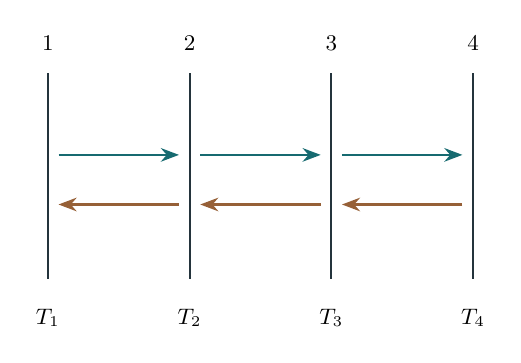
\begin{tikzpicture}[scale=.9,transform shape]
\draw[object] (0.00000,-1.30000)--(0.00000,1.60000);\node[above] at (0.00000,1.80000) {1};\node[below] at (0.00000,-1.60000) {$T_1$};\draw[motion] (0.15000,0.45000)--(1.85000,0.45000);\draw[force] (1.85000,-0.25000)--(0.15000,-0.25000);\draw[object] (2.00000,-1.30000)--(2.00000,1.60000);\node[above] at (2.00000,1.80000) {2};\node[below] at (2.00000,-1.60000) {$T_2$};\draw[motion] (2.15000,0.45000)--(3.85000,0.45000);\draw[force] (3.85000,-0.25000)--(2.15000,-0.25000);\draw[object] (4.00000,-1.30000)--(4.00000,1.60000);\node[above] at (4.00000,1.80000) {3};\node[below] at (4.00000,-1.60000) {$T_3$};\draw[motion] (4.15000,0.45000)--(5.85000,0.45000);\draw[force] (5.85000,-0.25000)--(4.15000,-0.25000);\draw[object] (6.00000,-1.30000)--(6.00000,1.60000);\node[above] at (6.00000,1.80000) {4};\node[below] at (6.00000,-1.60000) {$T_4$};
\end{tikzpicture}
\figcaption{图近1.4\quad 各间隙有相向辐射，中间板温度由平衡决定。}
\end{minipage}\end{center}

\workarea

\clearpage

\pdfbookmark[2]{第 5 题 真空包层下液氦的蒸发}{q5}

\section*{第 5 题\quad 真空包层下液氦的蒸发}\label{q:5}

黑色圆筒形容器直径$d=5.0\,\mathrm{cm}$、高$l=10.0\,\mathrm{cm}$，内盛沸点4.2K的液氦，汽化潜热$L_v=2.1\times10^4\,\mathrm{J/kg}$。侧壁及底部外包77K的绝热层，中间窄隙抽成真空。外包层在所涉及波段按漫灰体近似，发射率$\varepsilon=1/2$；两相对表面积近似相等。忽略开口、支撑、气体导热及其他热交换，汽化氦气立即逸出。取$\sigma=5.67\times10^{-8}\,\mathrm{W/(m^2K^4)}$，求每小时蒸发液氦质量。

\begin{center}\begin{minipage}{.98\linewidth}\centering
\begin{tikzpicture}[scale=.9,transform shape]
\draw[object] (0.00000,1.50000)--(0.00000,-1.50000)--(3.00000,-1.50000)--(3.00000,1.50000);\draw[object] (-0.35000,1.50000)--(-0.35000,-1.85000)--(3.35000,-1.85000)--(3.35000,1.50000);\node[above] at (1.50000,0.00000) {液氦 4.2K};\node[right] at (4.00000,0.00000) {包层77K};\node[right] at (4.00000,-0.70000) {窄真空间隙};\draw[<->,thin,color=muted] (0.00000,-2.40000)--(3.00000,-2.40000);\node[below] at (1.50000,-2.40000) {$d$};\draw[<->,thin,color=muted] (-1.00000,-1.50000)--(-1.00000,1.50000);\node[left] at (-1.00000,0.00000) {$l$};
\end{tikzpicture}
\figcaption{图近1.5\quad 侧壁和底面参与窄隙辐射交换，开口另行忽略。}
\end{minipage}\end{center}

\workarea

\clearpage

\pdfbookmark[2]{第 6 题 黑体谱峰的温度标度}{q6}

\section*{第 6 题\quad 黑体谱峰的温度标度}\label{q:6}

由普朗克黑体辐射公式证明：按每单位真空波长定义的平衡辐射能量密度谱$u_\lambda(T)$，其峰值与绝对温度的五次方成正比。推导峰位置，并说明若按每单位频率定义谱，峰值的温度幂次是否相同。

\begin{center}\begin{minipage}{.98\linewidth}\centering
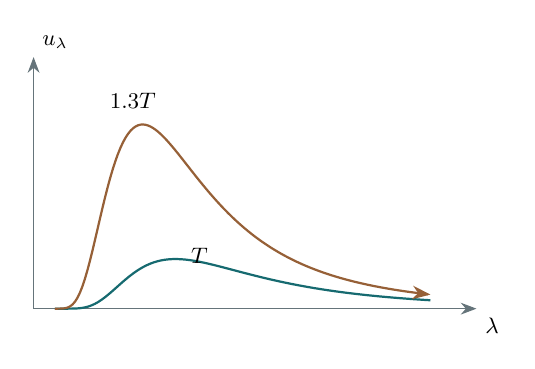
\begin{tikzpicture}[scale=.9,transform shape]
\draw[axis] (0.00000,0.00000)--(6.25000,0.00000);\draw[axis] (0.00000,0.00000)--(0.00000,3.55000);\node[below right] at (6.25000,0.00000) {$\lambda$};\node[above right] at (0.00000,3.55000) {$u_\lambda$};\draw[traj] plot coordinates {(0.30000,0.00000) (0.33557,0.00000) (0.37114,0.00000) (0.40671,0.00001) (0.44228,0.00003) (0.47785,0.00012) (0.51342,0.00036) (0.54899,0.00089) (0.58456,0.00196) (0.62013,0.00386) (0.65570,0.00696) (0.69128,0.01166) (0.72685,0.01832) (0.76242,0.02729) (0.79799,0.03883) (0.83356,0.05310) (0.86913,0.07016) (0.90470,0.08997) (0.94027,0.11238) (0.97584,0.13716) (1.01141,0.16403) (1.04698,0.19264) (1.08255,0.22261) (1.11812,0.25357) (1.15369,0.28512) (1.18926,0.31690) (1.22483,0.34855) (1.26040,0.37976) (1.29597,0.41023) (1.33154,0.43972) (1.36711,0.46800) (1.40268,0.49492) (1.43826,0.52031) (1.47383,0.54407) (1.50940,0.56613) (1.54497,0.58644) (1.58054,0.60496) (1.61611,0.62169) (1.65168,0.63665) (1.68725,0.64986) (1.72282,0.66138) (1.75839,0.67124) (1.79396,0.67952) (1.82953,0.68628) (1.86510,0.69160) (1.90067,0.69555) (1.93624,0.69821) (1.97181,0.69966) (2.00738,0.69998) (2.04295,0.69924) (2.07852,0.69753) (2.11409,0.69493) (2.14966,0.69149) (2.18523,0.68729) (2.22081,0.68240) (2.25638,0.67689) (2.29195,0.67081) (2.32752,0.66421) (2.36309,0.65716) (2.39866,0.64971) (2.43423,0.64190) (2.46980,0.63377) (2.50537,0.62537) (2.54094,0.61674) (2.57651,0.60791) (2.61208,0.59892) (2.64765,0.58979) (2.68322,0.58056) (2.71879,0.57125) (2.75436,0.56188) (2.78993,0.55247) (2.82550,0.54306) (2.86107,0.53364) (2.89664,0.52425) (2.93221,0.51489) (2.96779,0.50558) (3.00336,0.49633) (3.03893,0.48715) (3.07450,0.47805) (3.11007,0.46904) (3.14564,0.46013) (3.18121,0.45132) (3.21678,0.44263) (3.25235,0.43405) (3.28792,0.42558) (3.32349,0.41724) (3.35906,0.40903) (3.39463,0.40094) (3.43020,0.39299) (3.46577,0.38517) (3.50134,0.37748) (3.53691,0.36993) (3.57248,0.36251) (3.60805,0.35523) (3.64362,0.34808) (3.67919,0.34107) (3.71477,0.33419) (3.75034,0.32744) (3.78591,0.32083) (3.82148,0.31435) (3.85705,0.30800) (3.89262,0.30178) (3.92819,0.29568) (3.96376,0.28971) (3.99933,0.28387) (4.03490,0.27815) (4.07047,0.27254) (4.10604,0.26706) (4.14161,0.26169) (4.17718,0.25644) (4.21275,0.25130) (4.24832,0.24627) (4.28389,0.24135) (4.31946,0.23653) (4.35503,0.23182) (4.39060,0.22722) (4.42617,0.22271) (4.46174,0.21830) (4.49732,0.21399) (4.53289,0.20977) (4.56846,0.20565) (4.60403,0.20162) (4.63960,0.19767) (4.67517,0.19381) (4.71074,0.19004) (4.74631,0.18635) (4.78188,0.18274) (4.81745,0.17921) (4.85302,0.17576) (4.88859,0.17238) (4.92416,0.16908) (4.95973,0.16585) (4.99530,0.16269) (5.03087,0.15960) (5.06644,0.15658) (5.10201,0.15362) (5.13758,0.15073) (5.17315,0.14790) (5.20872,0.14514) (5.24430,0.14243) (5.27987,0.13978) (5.31544,0.13719) (5.35101,0.13466) (5.38658,0.13218) (5.42215,0.12975) (5.45772,0.12738) (5.49329,0.12506) (5.52886,0.12278) (5.56443,0.12056) (5.60000,0.11838)};\draw[force] plot coordinates {(0.30000,0.00001) (0.33557,0.00010) (0.37114,0.00052) (0.40671,0.00200) (0.44228,0.00595) (0.47785,0.01461) (0.51342,0.03089) (0.54899,0.05794) (0.58456,0.09870) (0.62013,0.15545) (0.65570,0.22944) (0.69128,0.32085) (0.72685,0.42875) (0.76242,0.55131) (0.79799,0.68603) (0.83356,0.82997) (0.86913,0.98000) (0.90470,1.13299) (0.94027,1.28599) (0.97584,1.43634) (1.01141,1.58171) (1.04698,1.72017) (1.08255,1.85019) (1.11812,1.97059) (1.15369,2.08055) (1.18926,2.17957) (1.22483,2.26741) (1.26040,2.34405) (1.29597,2.40967) (1.33154,2.46461) (1.36711,2.50928) (1.40268,2.54424) (1.43826,2.57005) (1.47383,2.58734) (1.50940,2.59675) (1.54497,2.59894) (1.58054,2.59453) (1.61611,2.58416) (1.65168,2.56843) (1.68725,2.54791) (1.72282,2.52314) (1.75839,2.49463) (1.79396,2.46286) (1.82953,2.42827) (1.86510,2.39126) (1.90067,2.35222) (1.93624,2.31147) (1.97181,2.26934) (2.00738,2.22609) (2.04295,2.18199) (2.07852,2.13727) (2.11409,2.09213) (2.14966,2.04674) (2.18523,2.00129) (2.22081,1.95590) (2.25638,1.91070) (2.29195,1.86581) (2.32752,1.82132) (2.36309,1.77732) (2.39866,1.73387) (2.43423,1.69105) (2.46980,1.64890) (2.50537,1.60746) (2.54094,1.56678) (2.57651,1.52688) (2.61208,1.48778) (2.64765,1.44950) (2.68322,1.41206) (2.71879,1.37546) (2.75436,1.33970) (2.78993,1.30480) (2.82550,1.27074) (2.86107,1.23753) (2.89664,1.20515) (2.93221,1.17360) (2.96779,1.14288) (3.00336,1.11295) (3.03893,1.08383) (3.07450,1.05548) (3.11007,1.02791) (3.14564,1.00108) (3.18121,0.97499) (3.21678,0.94963) (3.25235,0.92497) (3.28792,0.90100) (3.32349,0.87770) (3.35906,0.85505) (3.39463,0.83305) (3.43020,0.81167) (3.46577,0.79090) (3.50134,0.77071) (3.53691,0.75110) (3.57248,0.73205) (3.60805,0.71354) (3.64362,0.69556) (3.67919,0.67810) (3.71477,0.66113) (3.75034,0.64464) (3.78591,0.62862) (3.82148,0.61306) (3.85705,0.59794) (3.89262,0.58325) (3.92819,0.56898) (3.96376,0.55511) (3.99933,0.54163) (4.03490,0.52853) (4.07047,0.51580) (4.10604,0.50343) (4.14161,0.49140) (4.17718,0.47971) (4.21275,0.46835) (4.24832,0.45730) (4.28389,0.44656) (4.31946,0.43611) (4.35503,0.42596) (4.39060,0.41608) (4.42617,0.40647) (4.46174,0.39713) (4.49732,0.38804) (4.53289,0.37920) (4.56846,0.37059) (4.60403,0.36222) (4.63960,0.35407) (4.67517,0.34614) (4.71074,0.33843) (4.74631,0.33092) (4.78188,0.32360) (4.81745,0.31648) (4.85302,0.30955) (4.88859,0.30280) (4.92416,0.29623) (4.95973,0.28983) (4.99530,0.28359) (5.03087,0.27752) (5.06644,0.27160) (5.10201,0.26583) (5.13758,0.26021) (5.17315,0.25474) (5.20872,0.24940) (5.24430,0.24420) (5.27987,0.23913) (5.31544,0.23418) (5.35101,0.22936) (5.38658,0.22466) (5.42215,0.22008) (5.45772,0.21561) (5.49329,0.21125) (5.52886,0.20699) (5.56443,0.20284) (5.60000,0.19879)};\node[right] at (2.10000,0.75000) {$T$};\node[above] at (1.40000,2.70000) {$1.3T$};
\end{tikzpicture}
\figcaption{图近1.6\quad 同一波长坐标中的两温度普朗克谱。}
\end{minipage}\end{center}

\workarea

\clearpage

\pdfbookmark[2]{第 7 题 太阳照射下的卫星热平衡}{q7}

\section*{第 7 题\quad 太阳照射下的卫星热平衡}\label{q:7}

直径1m的球形卫星表面均温、覆同一种涂层，位于地球附近且始终在阳光中。太阳视为6000K黑体，半径$R_s=6.96\times10^8\,\mathrm m$，卫星距太阳$D=1.5\times10^{11}\,\mathrm m$。忽略地球辐射、反照、太空背景及导热。取$\sigma=5.67\times10^{-8}\,\mathrm{W/(m^2K^4)}$。
\begin{enumerate}[label=（\arabic*）]
\item 卫星也为黑体时，求平衡温度。
\item 改用理想不透光选择涂层：频率$f>f_c$全反射，$f<f_c$全吸收，其中$hf_c/k_B=1200\,\mathrm K$。依据普朗克谱估计温度；说明涂层的发射性质。可用$\int_0^\infty x^3/(e^x-1)\dd x=\pi^4/15$，小$x$时$e^x-1\simeq x$。
\item 同一选择涂层的卫星内部另有1kW持续热功率，求新的平衡温度。
\item 有人声称被动涂层能在所有可见、红外频率反射90\%以上，同时像黑体一样在所有频率发射，从而使卫星一直变冷。判断能否实现并说明理由。
\item 若要让无内部热源的卫星温度高于第（1）问的黑体温度，涂层应怎样选择吸收与发射频段？
\end{enumerate}

\begin{center}\begin{minipage}{.98\linewidth}\centering
\begin{tikzpicture}[scale=.9,transform shape]
\draw[object] (0.00000,0.00000) circle(0.75000);\node[above] at (0.00000,1.00000) {太阳 $T_s$};\draw[motion] (0.90000,0.35000)--(6.00000,0.35000);\draw[motion] (0.90000,-0.35000)--(6.00000,-0.35000);\draw[object] (6.50000,0.00000) circle(0.50000);\node[above] at (6.50000,1.00000) {卫星 $T$};\draw[<->,thin,color=muted] (0.00000,-1.20000)--(6.50000,-1.20000);\node[below] at (3.25000,-1.20000) {$D$};
\end{tikzpicture}
\figcaption{图近1.7\quad 太阳辐照度按距离平方稀释，卫星均温散热。}
\end{minipage}\end{center}

\workarea

\clearpage

\pdfbookmark[2]{第 8 题 由光电子磁轨道求逸出功}{q8}

\section*{第 8 题\quad 由光电子磁轨道求逸出功}\label{q:8}

波长350nm的光照射光电材料，逸出电子中动量最大的电子垂直进入$B=1.50\times10^{-5}\,\mathrm T$的匀强磁场，沿半径$r=18.0\,\mathrm{cm}$的圆轨道运动。磁场前无额外电势加速，求材料逸出功，检查所用电子动能近似。

\begin{center}\begin{minipage}{.98\linewidth}\centering
\begin{tikzpicture}[scale=.9,transform shape]
\draw[object] (0.00000,-1.80000)--(0.00000,1.10000);\node[above] at (0.00000,1.20000) {材料};\draw[traj] plot coordinates {(-2.00000,1.00000) (-1.98150,1.00939) (-1.96342,1.01737) (-1.94616,1.02263) (-1.93000,1.02421) (-1.91514,1.02147) (-1.90162,1.01426) (-1.88935,1.00288) (-1.87812,0.98806) (-1.86758,0.97089) (-1.85735,0.95271) (-1.84699,0.93496) (-1.83609,0.91903) (-1.82427,0.90614) (-1.81128,0.89716) (-1.79697,0.89259) (-1.78133,0.89246) (-1.76449,0.89632) (-1.74670,0.90333) (-1.72832,0.91231) (-1.70977,0.92188) (-1.69147,0.93060) (-1.67383,0.93711) (-1.65720,0.94028) (-1.64179,0.93935) (-1.62773,0.93396) (-1.61497,0.92421) (-1.60334,0.91068) (-1.59257,0.89432) (-1.58226,0.87638) (-1.57201,0.85828) (-1.56138,0.84145) (-1.54997,0.82719) (-1.53749,0.81653) (-1.52372,0.81014) (-1.50861,0.80822) (-1.49224,0.81053) (-1.47480,0.81638) (-1.45661,0.82472) (-1.43808,0.83422) (-1.41962,0.84346) (-1.40167,0.85102) (-1.38459,0.85567) (-1.36867,0.85649) (-1.35405,0.85293) (-1.34077,0.84491) (-1.32871,0.83283) (-1.31763,0.81749) (-1.30719,0.80003) (-1.29696,0.78182) (-1.28654,0.76430) (-1.27549,0.74885) (-1.26347,0.73662) (-1.25025,0.72843) (-1.23569,0.72469) (-1.21981,0.72534) (-1.20277,0.72985) (-1.18485,0.73732) (-1.16641,0.74651) (-1.14787,0.75604) (-1.12966,0.76444) (-1.11218,0.77042) (-1.09576,0.77289) (-1.08060,0.77115) (-1.06678,0.76493) (-1.05425,0.75443) (-1.04280,0.74030) (-1.03214,0.72355) (-1.02188,0.70547) (-1.01159,0.68750) (-1.00084,0.67105) (-0.98926,0.65739) (-0.97655,0.64747) (-0.96254,0.64190) (-0.94719,0.64079) (-0.93060,0.64382) (-0.91299,0.65021) (-0.89471,0.65887) (-0.87616,0.66843) (-0.85777,0.67746) (-0.83995,0.68457) (-0.82307,0.68858) (-0.80737,0.68862) (-0.79300,0.68423) (-0.77996,0.67543) (-0.76810,0.66267) (-0.75717,0.64685) (-0.74680,0.62914) (-0.73657,0.61095) (-0.72606,0.59372) (-0.71486,0.57878) (-0.70263,0.56724) (-0.68917,0.55986) (-0.67436,0.55694) (-0.65825,0.55835) (-0.64103,0.56348) (-0.62298,0.57137) (-0.60449,0.58073) (-0.58597,0.59016) (-0.56788,0.59821) (-0.55057,0.60361) (-0.53437,0.60534) (-0.51945,0.60279) (-0.50588,0.59576) (-0.49356,0.58453) (-0.48229,0.56983) (-0.47173,0.55273) (-0.46150,0.53457) (-0.45116,0.51677) (-0.44028,0.50074) (-0.42851,0.48771) (-0.41557,0.47856) (-0.40131,0.47381) (-0.38572,0.47350) (-0.36892,0.47722) (-0.35117,0.48412) (-0.33281,0.49305) (-0.31425,0.50262) (-0.29593,0.51140) (-0.27826,0.51802) (-0.26158,0.52135) (-0.24612,0.52060) (-0.23200,0.51538) (-0.21919,0.50581) (-0.20753,0.49241) (-0.19673,0.47614) (-0.18641,0.45824) (-0.17617,0.44012) (-0.16555,0.42321) (-0.15419,0.40882) (-0.14175,0.39801) (-0.12804,0.39143) (-0.11298,0.38933) (-0.09666,0.39148) (-0.07925,0.39721) (-0.06109,0.40547) (-0.04256,0.41495) (-0.02410,0.42423) (-0.00612,0.43188) (0.01100,0.43668)};\draw[motion] (-0.17241,0.45172)--(0.00000,0.40000);\node[above] at (-1.00000,0.70000) {350nm};\draw[motion] (0.00000,0.00000)--(2.50000,0.00000);\draw[traj] plot coordinates {(2.50000,0.00000) (2.54751,-0.00094) (2.59494,-0.00376) (2.64222,-0.00846) (2.68929,-0.01502) (2.73605,-0.02345) (2.78244,-0.03371) (2.82840,-0.04581) (2.87383,-0.05972) (2.91868,-0.07541) (2.96288,-0.09287) (3.00634,-0.11206) (3.04902,-0.13296) (3.09083,-0.15553) (3.13172,-0.17974) (3.17162,-0.20555) (3.21046,-0.23292) (3.24819,-0.26180) (3.28474,-0.29216) (3.32007,-0.32394) (3.35411,-0.35709) (3.38681,-0.39157) (3.41812,-0.42731) (3.44799,-0.46426) (3.47638,-0.50237) (3.50323,-0.54157) (3.52851,-0.58180) (3.55218,-0.62301) (3.57420,-0.66511) (3.59453,-0.70806) (3.61315,-0.75178) (3.63002,-0.79620) (3.64512,-0.84125) (3.65842,-0.88687) (3.66991,-0.93297) (3.67957,-0.97950) (3.68737,-1.02637) (3.69332,-1.07352) (3.69739,-1.12086) (3.69958,-1.16832) (3.69990,-1.21584) (3.69833,-1.26333) (3.69488,-1.31072) (3.68956,-1.35794) (3.68238,-1.40491) (3.67334,-1.45156) (3.66246,-1.49781) (3.64976,-1.54360) (3.63525,-1.58885) (3.61897,-1.63349) (3.60093,-1.67745) (3.58116,-1.72066) (3.55970,-1.76306) (3.53658,-1.80457) (3.51183,-1.84513) (3.48550,-1.88468) (3.45762,-1.92316) (3.42824,-1.96051) (3.39740,-1.99666) (3.36516,-2.03156) (3.33156,-2.06516) (3.29666,-2.09740) (3.26051,-2.12824) (3.22316,-2.15762) (3.18468,-2.18550) (3.14513,-2.21183) (3.10457,-2.23658) (3.06306,-2.25970) (3.02066,-2.28116) (2.97745,-2.30093) (2.93349,-2.31897) (2.88885,-2.33525) (2.84360,-2.34976) (2.79781,-2.36246) (2.75156,-2.37334) (2.70491,-2.38238) (2.65794,-2.38956) (2.61072,-2.39488) (2.56333,-2.39833) (2.51584,-2.39990) (2.46832,-2.39958) (2.42086,-2.39739) (2.37352,-2.39332) (2.32637,-2.38737) (2.27950,-2.37957) (2.23297,-2.36991) (2.18687,-2.35842) (2.14125,-2.34512) (2.09620,-2.33002) (2.05178,-2.31315) (2.00806,-2.29453) (1.96511,-2.27420) (1.92301,-2.25218) (1.88180,-2.22851) (1.84157,-2.20323) (1.80237,-2.17638) (1.76426,-2.14799) (1.72731,-2.11812) (1.69157,-2.08681) (1.65709,-2.05411) (1.62394,-2.02007) (1.59216,-1.98474) (1.56180,-1.94819) (1.53292,-1.91046) (1.50555,-1.87162) (1.47974,-1.83172) (1.45553,-1.79083) (1.43296,-1.74902) (1.41206,-1.70634) (1.39287,-1.66288) (1.37541,-1.61868) (1.35972,-1.57383) (1.34581,-1.52840) (1.33371,-1.48244) (1.32345,-1.43605) (1.31502,-1.38929) (1.30846,-1.34222) (1.30376,-1.29494) (1.30094,-1.24751) (1.30000,-1.20000)};\draw[motion] (3.68000,-1.00000)--(3.68000,-1.35000);\draw[<->,thin,color=muted] (2.50000,-1.20000)--(1.30000,-1.20000);\node[below] at (1.90000,-1.20000) {$r$};\draw[force] (2.50000,0.00000)--(2.50000,-0.65000);\node[right] at (2.70000,-0.50000) {$\boldsymbol F_B$};\node[above] at (1.20000,-1.80000) {$\otimes$};\node[above] at (1.20000,-0.30000) {$\otimes$};\node[above] at (4.30000,-1.80000) {$\otimes$};\node[above] at (4.30000,-0.30000) {$\otimes$};\node[above] at (4.50000,1.00000) {$B$入纸面};\node[above] at (0.80000,0.25000) {$\boldsymbol p$};
\end{tikzpicture}
\figcaption{图近1.8\quad 光电子逸出后进入匀强磁场，磁力不做功。}
\end{minipage}\end{center}

\workarea

\clearpage

\pdfbookmark[2]{第 9 题 自由电子为何不能完整吸收单光子}{q9}

\section*{第 9 题\quad 自由电子为何不能完整吸收单光子}\label{q:9}

证明孤立、起初静止的自由电子不可能完整吸收一个非零能量光子后仍成为同一种自由电子。要求同时使用能量和动量守恒，并解释束缚电子产生光电效应为何不矛盾。

\begin{center}\begin{minipage}{.98\linewidth}\centering
\begin{tikzpicture}[scale=.9,transform shape]
\draw[traj] plot coordinates {(-2.00000,0.00000) (-1.98561,0.01432) (-1.97122,0.02714) (-1.95683,0.03715) (-1.94245,0.04330) (-1.92806,0.04495) (-1.91367,0.04193) (-1.89928,0.03455) (-1.88489,0.02358) (-1.87050,0.01017) (-1.85612,-0.00431) (-1.84173,-0.01833) (-1.82734,-0.03045) (-1.81295,-0.03941) (-1.79856,-0.04427) (-1.78417,-0.04454) (-1.76978,-0.04017) (-1.75540,-0.03163) (-1.74101,-0.01981) (-1.72662,-0.00593) (-1.71223,0.00857) (-1.69784,0.02218) (-1.68345,0.03348) (-1.66906,0.04131) (-1.65468,0.04484) (-1.64029,0.04372) (-1.62590,0.03805) (-1.61151,0.02843) (-1.59712,0.01585) (-1.58273,0.00163) (-1.56835,-0.01276) (-1.55396,-0.02582) (-1.53957,-0.03621) (-1.52518,-0.04283) (-1.51079,-0.04500) (-1.49640,-0.04249) (-1.48201,-0.03557) (-1.46763,-0.02496) (-1.45324,-0.01175) (-1.43885,0.00268) (-1.42446,0.01683) (-1.41007,0.02923) (-1.39568,0.03860) (-1.38129,0.04395) (-1.36691,0.04474) (-1.35252,0.04088) (-1.33813,0.03277) (-1.32374,0.02126) (-1.30935,0.00754) (-1.29496,-0.00696) (-1.28058,-0.02074) (-1.26619,-0.03237) (-1.25180,-0.04063) (-1.23741,-0.04467) (-1.22302,-0.04407) (-1.20863,-0.03889) (-1.19424,-0.02967) (-1.17986,-0.01737) (-1.16547,-0.00326) (-1.15108,0.01118) (-1.13669,0.02447) (-1.12230,0.03521) (-1.10791,0.04230) (-1.09353,0.04499) (-1.07914,0.04300) (-1.06475,0.03655) (-1.05036,0.02630) (-1.03597,0.01332) (-1.02158,-0.00105) (-1.00719,-0.01530) (-0.99281,-0.02797) (-0.97842,-0.03773) (-0.96403,-0.04357) (-0.94964,-0.04489) (-0.93525,-0.04154) (-0.92086,-0.03387) (-0.90647,-0.02269) (-0.89209,-0.00915) (-0.87770,0.00534) (-0.86331,0.01928) (-0.84892,0.03121) (-0.83453,0.03990) (-0.82014,0.04445) (-0.80576,0.04437) (-0.79137,0.03969) (-0.77698,0.03088) (-0.76259,0.01887) (-0.74820,0.00489) (-0.73381,-0.00960) (-0.71942,-0.02308) (-0.70504,-0.03417) (-0.69065,-0.04171) (-0.67626,-0.04492) (-0.66187,-0.04346) (-0.64748,-0.03748) (-0.63309,-0.02761) (-0.61871,-0.01487) (-0.60432,-0.00059) (-0.58993,0.01376) (-0.57554,0.02667) (-0.56115,0.03682) (-0.54676,0.04314) (-0.53237,0.04497) (-0.51799,0.04214) (-0.50360,0.03492) (-0.48921,0.02408) (-0.47482,0.01074) (-0.46043,-0.00372) (-0.44604,-0.01779) (-0.43165,-0.03002) (-0.41727,-0.03912) (-0.40288,-0.04416) (-0.38849,-0.04462) (-0.37410,-0.04043) (-0.35971,-0.03205) (-0.34532,-0.02034) (-0.33094,-0.00651) (-0.31655,0.00799) (-0.30216,0.02167) (-0.28777,0.03309) (-0.27338,0.04107) (-0.25899,0.04479) (-0.24460,0.04385) (-0.23022,0.03836) (-0.21583,0.02888) (-0.20144,0.01640) (-0.18705,0.00222) (-0.17266,-0.01219) (-0.15827,-0.02534) (-0.14388,-0.03585) (-0.12950,-0.04264) (-0.11511,-0.04500) (-0.10072,-0.04268) (-0.08633,-0.03593) (-0.07194,-0.02545) (-0.05755,-0.01232) (-0.04317,0.00209) (-0.02878,0.01628) (-0.01439,0.02878) (0.00000,0.03829)};\draw[motion] (-0.18000,0.00000)--(0.00000,0.00000);\node[above] at (-1.00000,0.00000) {$E_\gamma,\ E_\gamma/c$};\fill (0.00000,0.00000) circle(.035);\node[below] at (0.00000,0.00000) {$e^-$};\node[above] at (0.00000,0.50000) {初始静止};\draw[force] (0.70000,0.00000)--(4.00000,0.00000);\node[above] at (3.00000,0.20000) {假设：只剩一个电子};
\end{tikzpicture}
\figcaption{图近1.9\quad 假定末态只有一个同质量自由电子。}
\end{minipage}\end{center}

\workarea

\clearpage

\pdfbookmark[2]{第 10 题 已知散射波长的康普顿反冲}{q10}

\section*{第 10 题\quad 已知散射波长的康普顿反冲}\label{q:10}

光子与起初静止的自由电子发生康普顿散射。散射光与入射光夹角为60°，散射光真空波长$\lambda'=0.0254\,\mathrm{nm}$。求反冲电子的动能和动量，并由守恒式确定反冲方向。可取$\lambda_C=h/(m_ec)=0.00242631\,\mathrm{nm}$、$hc=1239.84\,\mathrm{eV\,nm}$、$m_ec^2=510999\,\mathrm{eV}$。

\begin{center}\begin{minipage}{.98\linewidth}\centering
\begin{tikzpicture}[scale=.9,transform shape]
\fill (0.00000,0.00000) circle(.035);\node[below left] at (0.00000,0.00000) {$O$};\draw[guide] (0.00000,0.00000)--(3.50000,0.00000);\draw[traj] plot coordinates {(-2.80000,0.00000) (-2.77986,0.01432) (-2.75971,0.02714) (-2.73957,0.03715) (-2.71942,0.04330) (-2.69928,0.04495) (-2.67914,0.04193) (-2.65899,0.03455) (-2.63885,0.02358) (-2.61871,0.01017) (-2.59856,-0.00431) (-2.57842,-0.01833) (-2.55827,-0.03045) (-2.53813,-0.03941) (-2.51799,-0.04427) (-2.49784,-0.04454) (-2.47770,-0.04017) (-2.45755,-0.03163) (-2.43741,-0.01981) (-2.41727,-0.00593) (-2.39712,0.00857) (-2.37698,0.02218) (-2.35683,0.03348) (-2.33669,0.04131) (-2.31655,0.04484) (-2.29640,0.04372) (-2.27626,0.03805) (-2.25612,0.02843) (-2.23597,0.01585) (-2.21583,0.00163) (-2.19568,-0.01276) (-2.17554,-0.02582) (-2.15540,-0.03621) (-2.13525,-0.04283) (-2.11511,-0.04500) (-2.09496,-0.04249) (-2.07482,-0.03557) (-2.05468,-0.02496) (-2.03453,-0.01175) (-2.01439,0.00268) (-1.99424,0.01683) (-1.97410,0.02923) (-1.95396,0.03860) (-1.93381,0.04395) (-1.91367,0.04474) (-1.89353,0.04088) (-1.87338,0.03277) (-1.85324,0.02126) (-1.83309,0.00754) (-1.81295,-0.00696) (-1.79281,-0.02074) (-1.77266,-0.03237) (-1.75252,-0.04063) (-1.73237,-0.04467) (-1.71223,-0.04407) (-1.69209,-0.03889) (-1.67194,-0.02967) (-1.65180,-0.01737) (-1.63165,-0.00326) (-1.61151,0.01118) (-1.59137,0.02447) (-1.57122,0.03521) (-1.55108,0.04230) (-1.53094,0.04499) (-1.51079,0.04300) (-1.49065,0.03655) (-1.47050,0.02630) (-1.45036,0.01332) (-1.43022,-0.00105) (-1.41007,-0.01530) (-1.38993,-0.02797) (-1.36978,-0.03773) (-1.34964,-0.04357) (-1.32950,-0.04489) (-1.30935,-0.04154) (-1.28921,-0.03387) (-1.26906,-0.02269) (-1.24892,-0.00915) (-1.22878,0.00534) (-1.20863,0.01928) (-1.18849,0.03121) (-1.16835,0.03990) (-1.14820,0.04445) (-1.12806,0.04437) (-1.10791,0.03969) (-1.08777,0.03088) (-1.06763,0.01887) (-1.04748,0.00489) (-1.02734,-0.00960) (-1.00719,-0.02308) (-0.98705,-0.03417) (-0.96691,-0.04171) (-0.94676,-0.04492) (-0.92662,-0.04346) (-0.90647,-0.03748) (-0.88633,-0.02761) (-0.86619,-0.01487) (-0.84604,-0.00059) (-0.82590,0.01376) (-0.80576,0.02667) (-0.78561,0.03682) (-0.76547,0.04314) (-0.74532,0.04497) (-0.72518,0.04214) (-0.70504,0.03492) (-0.68489,0.02408) (-0.66475,0.01074) (-0.64460,-0.00372) (-0.62446,-0.01779) (-0.60432,-0.03002) (-0.58417,-0.03912) (-0.56403,-0.04416) (-0.54388,-0.04462) (-0.52374,-0.04043) (-0.50360,-0.03205) (-0.48345,-0.02034) (-0.46331,-0.00651) (-0.44317,0.00799) (-0.42302,0.02167) (-0.40288,0.03309) (-0.38273,0.04107) (-0.36259,0.04479) (-0.34245,0.04385) (-0.32230,0.03836) (-0.30216,0.02888) (-0.28201,0.01640) (-0.26187,0.00222) (-0.24173,-0.01219) (-0.22158,-0.02534) (-0.20144,-0.03585) (-0.18129,-0.04264) (-0.16115,-0.04500) (-0.14101,-0.04268) (-0.12086,-0.03593) (-0.10072,-0.02545) (-0.08058,-0.01232) (-0.06043,0.00209) (-0.04029,0.01628) (-0.02014,0.02878) (0.00000,0.03829)};\draw[motion] (-0.18000,0.00000)--(0.00000,0.00000);\node[above] at (-1.40000,0.00000) {$h/\lambda$};\draw[traj] plot coordinates {(0.00000,0.00000) (-0.00233,0.02460) (-0.00336,0.04846) (-0.00196,0.07091) (0.00279,0.09143) (0.01143,0.10970) (0.02412,0.12563) (0.04058,0.13939) (0.06015,0.15135) (0.08184,0.16209) (0.10445,0.17230) (0.12667,0.18273) (0.14724,0.19412) (0.16507,0.20708) (0.17935,0.22210) (0.18965,0.23941) (0.19594,0.25904) (0.19862,0.28075) (0.19845,0.30411) (0.19650,0.32849) (0.19402,0.35319) (0.19230,0.37744) (0.19259,0.40053) (0.19588,0.42189) (0.20289,0.44110) (0.21394,0.45799) (0.22892,0.47260) (0.24732,0.48523) (0.26828,0.49639) (0.29067,0.50672) (0.31321,0.51697) (0.33459,0.52789) (0.35366,0.54014) (0.36946,0.55428) (0.38141,0.57064) (0.38932,0.58933) (0.39340,0.61024) (0.39428,0.63299) (0.39291,0.65704) (0.39049,0.68170) (0.38830,0.70622) (0.38764,0.72986) (0.38960,0.75199) (0.39503,0.77212) (0.40442,0.78996) (0.41783,0.80547) (0.43493,0.81886) (0.45497,0.83055) (0.47692,0.84114) (0.49955,0.85133) (0.52156,0.86188) (0.54170,0.87352) (0.55893,0.88683) (0.57250,0.90225) (0.58205,0.92000) (0.58764,0.94003) (0.58973,0.96209) (0.58914,0.98569) (0.58700,1.01019) (0.58456,1.03485) (0.58313,1.05894) (0.58389,1.08176) (0.58783,1.10275) (0.59557,1.12154) (0.60736,1.13799) (0.62302,1.15221) (0.64197,1.16453) (0.66328,1.17548) (0.68580,1.18575) (0.70822,1.19606) (0.72926,1.20717) (0.74778,1.21974) (0.76291,1.23426) (0.77412,1.25105) (0.78130,1.27017) (0.78473,1.29145) (0.78512,1.31448) (0.78346,1.33870) (0.78098,1.36339) (0.77899,1.38780) (0.77872,1.41122) (0.78127,1.43301) (0.78741,1.45272) (0.79754,1.47013) (0.81167,1.48523) (0.82937,1.49828) (0.84985,1.50971) (0.87202,1.52017) (0.89464,1.53037) (0.91639,1.54107) (0.93607,1.55297) (0.95267,1.56665) (0.96552,1.58249) (0.97432,1.60067) (0.97922,1.62110) (0.98074,1.64348) (0.97978,1.66730) (0.97749,1.69188) (0.97514,1.71650) (0.97402,1.74040) (0.97531,1.76292) (0.97991,1.78352) (0.98839,1.80189) (1.00092,1.81792) (1.01724,1.83175) (1.03670,1.84378) (1.05833,1.85455) (1.08092,1.86477) (1.10318,1.87518) (1.12384,1.88651) (1.14180,1.89940) (1.15623,1.91433) (1.16670,1.93154) (1.17315,1.95108) (1.17596,1.97272) (1.17588,1.99602) (1.17398,2.02038) (1.17149,2.04508) (1.16973,2.06936) (1.16991,2.09251) (1.17306,2.11395) (1.17992,2.13325) (1.19080,2.15023) (1.20563,2.16493) (1.22391,2.17763) (1.24479,2.18884) (1.26714,2.19919) (1.28970,2.20943) (1.31115,2.22030) (1.33033,2.23249) (1.34628,2.24654) (1.35840,2.26281) (1.36646,2.28141) (1.37069,2.30223) (1.37168,2.32492) (1.37038,2.34893) (1.36797,2.37358) (1.36576,2.39812) (1.36500,2.42182) (1.36684,2.44402)};\draw[motion] (1.31000,2.26899)--(1.40000,2.42487);\node[above] at (0.70000,1.21244) {$h/\lambda'$};\draw[force] (0.00000,0.00000)--(1.23330,-1.94138);\node[below right] at (1.23330,-1.94138) {$p_e$};\node[above] at (0.70000,0.35000) {$\theta$};\node[below] at (0.95000,-0.10000) {$\varphi$};\draw[guide] plot coordinates {(0.42897,-0.67526) (0.45806,-0.65588) (0.48627,-0.63525) (0.51355,-0.61341) (0.53985,-0.59039) (0.56512,-0.56625) (0.58931,-0.54103) (0.61238,-0.51478) (0.63427,-0.48754) (0.65496,-0.45937) (0.67440,-0.43033) (0.69255,-0.40046) (0.70938,-0.36983) (0.72486,-0.33850) (0.73895,-0.30652) (0.75163,-0.27395) (0.76288,-0.24086) (0.77267,-0.20731) (0.78099,-0.17337) (0.78782,-0.13909) (0.79314,-0.10455) (0.79695,-0.06981) (0.79924,-0.03494) (0.80000,0.00000)};
\end{tikzpicture}
\figcaption{图近1.10\quad 光子向上散射，电子向下反冲，横向动量相消。}
\end{minipage}\end{center}

\workarea

\clearpage

\pdfbookmark[2]{第 11 题 由电子反冲方向求能量}{q11}

\section*{第 11 题\quad 由电子反冲方向求能量}\label{q:11}

光子频率$\nu$与起初静止的自由电子发生康普顿散射。已知反冲电子的运动方向与光子入射方向夹角为$\varphi$，求电子动能；说明物理允许的角度、零反冲退化和最大动能。

\begin{center}\begin{minipage}{.98\linewidth}\centering
\begin{tikzpicture}[scale=.9,transform shape]
\fill (0.00000,0.00000) circle(.035);\node[below left] at (0.00000,0.00000) {$O$};\draw[guide] (0.00000,0.00000)--(3.50000,0.00000);\draw[traj] plot coordinates {(-2.80000,0.00000) (-2.77986,0.01432) (-2.75971,0.02714) (-2.73957,0.03715) (-2.71942,0.04330) (-2.69928,0.04495) (-2.67914,0.04193) (-2.65899,0.03455) (-2.63885,0.02358) (-2.61871,0.01017) (-2.59856,-0.00431) (-2.57842,-0.01833) (-2.55827,-0.03045) (-2.53813,-0.03941) (-2.51799,-0.04427) (-2.49784,-0.04454) (-2.47770,-0.04017) (-2.45755,-0.03163) (-2.43741,-0.01981) (-2.41727,-0.00593) (-2.39712,0.00857) (-2.37698,0.02218) (-2.35683,0.03348) (-2.33669,0.04131) (-2.31655,0.04484) (-2.29640,0.04372) (-2.27626,0.03805) (-2.25612,0.02843) (-2.23597,0.01585) (-2.21583,0.00163) (-2.19568,-0.01276) (-2.17554,-0.02582) (-2.15540,-0.03621) (-2.13525,-0.04283) (-2.11511,-0.04500) (-2.09496,-0.04249) (-2.07482,-0.03557) (-2.05468,-0.02496) (-2.03453,-0.01175) (-2.01439,0.00268) (-1.99424,0.01683) (-1.97410,0.02923) (-1.95396,0.03860) (-1.93381,0.04395) (-1.91367,0.04474) (-1.89353,0.04088) (-1.87338,0.03277) (-1.85324,0.02126) (-1.83309,0.00754) (-1.81295,-0.00696) (-1.79281,-0.02074) (-1.77266,-0.03237) (-1.75252,-0.04063) (-1.73237,-0.04467) (-1.71223,-0.04407) (-1.69209,-0.03889) (-1.67194,-0.02967) (-1.65180,-0.01737) (-1.63165,-0.00326) (-1.61151,0.01118) (-1.59137,0.02447) (-1.57122,0.03521) (-1.55108,0.04230) (-1.53094,0.04499) (-1.51079,0.04300) (-1.49065,0.03655) (-1.47050,0.02630) (-1.45036,0.01332) (-1.43022,-0.00105) (-1.41007,-0.01530) (-1.38993,-0.02797) (-1.36978,-0.03773) (-1.34964,-0.04357) (-1.32950,-0.04489) (-1.30935,-0.04154) (-1.28921,-0.03387) (-1.26906,-0.02269) (-1.24892,-0.00915) (-1.22878,0.00534) (-1.20863,0.01928) (-1.18849,0.03121) (-1.16835,0.03990) (-1.14820,0.04445) (-1.12806,0.04437) (-1.10791,0.03969) (-1.08777,0.03088) (-1.06763,0.01887) (-1.04748,0.00489) (-1.02734,-0.00960) (-1.00719,-0.02308) (-0.98705,-0.03417) (-0.96691,-0.04171) (-0.94676,-0.04492) (-0.92662,-0.04346) (-0.90647,-0.03748) (-0.88633,-0.02761) (-0.86619,-0.01487) (-0.84604,-0.00059) (-0.82590,0.01376) (-0.80576,0.02667) (-0.78561,0.03682) (-0.76547,0.04314) (-0.74532,0.04497) (-0.72518,0.04214) (-0.70504,0.03492) (-0.68489,0.02408) (-0.66475,0.01074) (-0.64460,-0.00372) (-0.62446,-0.01779) (-0.60432,-0.03002) (-0.58417,-0.03912) (-0.56403,-0.04416) (-0.54388,-0.04462) (-0.52374,-0.04043) (-0.50360,-0.03205) (-0.48345,-0.02034) (-0.46331,-0.00651) (-0.44317,0.00799) (-0.42302,0.02167) (-0.40288,0.03309) (-0.38273,0.04107) (-0.36259,0.04479) (-0.34245,0.04385) (-0.32230,0.03836) (-0.30216,0.02888) (-0.28201,0.01640) (-0.26187,0.00222) (-0.24173,-0.01219) (-0.22158,-0.02534) (-0.20144,-0.03585) (-0.18129,-0.04264) (-0.16115,-0.04500) (-0.14101,-0.04268) (-0.12086,-0.03593) (-0.10072,-0.02545) (-0.08058,-0.01232) (-0.06043,0.00209) (-0.04029,0.01628) (-0.02014,0.02878) (0.00000,0.03829)};\draw[motion] (-0.18000,0.00000)--(0.00000,0.00000);\node[above] at (-1.40000,0.00000) {$h/\lambda$};\draw[traj] plot coordinates {(0.00000,0.00000) (-0.00656,0.02383) (-0.01173,0.04714) (-0.01424,0.06949) (-0.01313,0.09053) (-0.00779,0.11002) (0.00194,0.12791) (0.01576,0.14432) (0.03295,0.15950) (0.05245,0.17384) (0.07294,0.18782) (0.09301,0.20195) (0.11129,0.21673) (0.12660,0.23260) (0.13806,0.24986) (0.14519,0.26870) (0.14798,0.28913) (0.14685,0.31097) (0.14263,0.33395) (0.13647,0.35762) (0.12974,0.38151) (0.12384,0.40510) (0.12011,0.42789) (0.11964,0.44950) (0.12321,0.46963) (0.13116,0.48818) (0.14338,0.50517) (0.15931,0.52081) (0.17801,0.53544) (0.19826,0.54950) (0.21868,0.56351) (0.23784,0.57797) (0.25449,0.59335) (0.26760,0.61001) (0.27653,0.62820) (0.28107,0.64798) (0.28146,0.66928) (0.27837,0.69184) (0.27285,0.71528) (0.26618,0.73915) (0.25977,0.76292) (0.25501,0.78609) (0.25310,0.80822) (0.25495,0.82898) (0.26110,0.84818) (0.27162,0.86579) (0.28612,0.88195) (0.30383,0.89694) (0.32361,0.91117) (0.34413,0.92514) (0.36397,0.93936) (0.38179,0.95431) (0.39644,0.97041) (0.40713,0.98796) (0.41345,1.00710) (0.41548,1.02780) (0.41370,1.04988) (0.40903,1.07302) (0.40266,1.09677) (0.39598,1.12064) (0.39038,1.14411) (0.38718,1.16672) (0.38741,1.18807) (0.39177,1.20792) (0.40053,1.22617) (0.41348,1.24289) (0.43000,1.25831) (0.44909,1.27280) (0.46948,1.28682) (0.48976,1.30087) (0.50856,1.31547) (0.52462,1.33106) (0.53700,1.34799) (0.54512,1.36647) (0.54886,1.38654) (0.54855,1.40809) (0.54493,1.43085) (0.53910,1.45441) (0.53237,1.47829) (0.52616,1.50199) (0.52184,1.52500) (0.52056,1.54690) (0.52318,1.56739) (0.53014,1.58629) (0.54143,1.60362) (0.55660,1.61953) (0.57478,1.63435) (0.59480,1.64850) (0.61530,1.66248) (0.63487,1.67679) (0.65218,1.69193) (0.66615,1.70828) (0.67605,1.72611) (0.68157,1.74554) (0.68284,1.76651) (0.68046,1.78882) (0.67538,1.81210) (0.66884,1.83592) (0.66225,1.85975) (0.65701,1.88310) (0.65437,1.90550) (0.65532,1.92659) (0.66048,1.94615) (0.67003,1.96411) (0.68370,1.98057) (0.70078,1.99579) (0.72021,2.01015) (0.74068,2.02414) (0.76080,2.03825) (0.77918,2.05300) (0.79462,2.06882) (0.80625,2.08602) (0.81356,2.10480) (0.81652,2.12515) (0.81553,2.14695) (0.81141,2.16989) (0.80531,2.19354) (0.79857,2.21743) (0.79262,2.24104) (0.78877,2.26387) (0.78816,2.28553) (0.79156,2.30573) (0.79933,2.32434) (0.81138,2.34139) (0.82717,2.35708) (0.84579,2.37174) (0.86601,2.38582) (0.88644,2.39982) (0.90568,2.41425) (0.92245,2.42959) (0.93572,2.44619) (0.94483,2.46432) (0.94954,2.48404) (0.95008,2.50528) (0.94712,2.52779) (0.94167,2.55121) (0.93502,2.57507) (0.92858,2.59885) (0.92372,2.62205) (0.92167,2.64424)};\draw[motion] (0.89609,2.46199)--(0.95766,2.63114);\node[above] at (0.47883,1.31557) {$h/\lambda'$};\draw[force] (0.00000,0.00000)--(1.46674,-1.77163);\node[below right] at (1.46674,-1.77163) {$p_e$};\node[above] at (0.70000,0.35000) {$\theta$};\node[below] at (0.95000,-0.10000) {$\varphi$};\draw[guide] plot coordinates {(0.51017,-0.61622) (0.53335,-0.59627) (0.55575,-0.57545) (0.57734,-0.55379) (0.59808,-0.53132) (0.61795,-0.50807) (0.63692,-0.48408) (0.65495,-0.45938) (0.67203,-0.43402) (0.68813,-0.40801) (0.70322,-0.38142) (0.71729,-0.35426) (0.73030,-0.32659) (0.74225,-0.29844) (0.75311,-0.26985) (0.76288,-0.24087) (0.77153,-0.21154) (0.77905,-0.18189) (0.78543,-0.15199) (0.79066,-0.12186) (0.79474,-0.09155) (0.79766,-0.06111) (0.79942,-0.03058) (0.80000,0.00000)};
\end{tikzpicture}
\figcaption{图近1.11\quad 电子方向角为已知，光子出射方向由守恒确定。}
\end{minipage}\end{center}

\workarea

\clearpage

\pdfbookmark[2]{第 12 题 最大能量转移反求入射波长}{q12}

\section*{第 12 题\quad 最大能量转移反求入射波长}\label{q:12}

一次光子与静止自由电子的康普顿散射中，可传给电子的最大动能为$K_{\max}=4.5\times10^4\,\mathrm{eV}$。求入射光子真空波长。取$m_ec^2=510999\,\mathrm{eV}$、$hc=1239.84\,\mathrm{eV\,nm}$。

\begin{center}\begin{minipage}{.98\linewidth}\centering
\begin{tikzpicture}[scale=.9,transform shape]
\draw[traj] plot coordinates {(-3.00000,1.00000) (-2.97842,1.01432) (-2.95683,1.02714) (-2.93525,1.03715) (-2.91367,1.04330) (-2.89209,1.04495) (-2.87050,1.04193) (-2.84892,1.03455) (-2.82734,1.02358) (-2.80576,1.01017) (-2.78417,0.99569) (-2.76259,0.98167) (-2.74101,0.96955) (-2.71942,0.96059) (-2.69784,0.95573) (-2.67626,0.95546) (-2.65468,0.95983) (-2.63309,0.96837) (-2.61151,0.98019) (-2.58993,0.99407) (-2.56835,1.00857) (-2.54676,1.02218) (-2.52518,1.03348) (-2.50360,1.04131) (-2.48201,1.04484) (-2.46043,1.04372) (-2.43885,1.03805) (-2.41727,1.02843) (-2.39568,1.01585) (-2.37410,1.00163) (-2.35252,0.98724) (-2.33094,0.97418) (-2.30935,0.96379) (-2.28777,0.95717) (-2.26619,0.95500) (-2.24460,0.95751) (-2.22302,0.96443) (-2.20144,0.97504) (-2.17986,0.98825) (-2.15827,1.00268) (-2.13669,1.01683) (-2.11511,1.02923) (-2.09353,1.03860) (-2.07194,1.04395) (-2.05036,1.04474) (-2.02878,1.04088) (-2.00719,1.03277) (-1.98561,1.02126) (-1.96403,1.00754) (-1.94245,0.99304) (-1.92086,0.97926) (-1.89928,0.96763) (-1.87770,0.95937) (-1.85612,0.95533) (-1.83453,0.95593) (-1.81295,0.96111) (-1.79137,0.97033) (-1.76978,0.98263) (-1.74820,0.99674) (-1.72662,1.01118) (-1.70504,1.02447) (-1.68345,1.03521) (-1.66187,1.04230) (-1.64029,1.04499) (-1.61871,1.04300) (-1.59712,1.03655) (-1.57554,1.02630) (-1.55396,1.01332) (-1.53237,0.99895) (-1.51079,0.98470) (-1.48921,0.97203) (-1.46763,0.96227) (-1.44604,0.95643) (-1.42446,0.95511) (-1.40288,0.95846) (-1.38129,0.96613) (-1.35971,0.97731) (-1.33813,0.99085) (-1.31655,1.00534) (-1.29496,1.01928) (-1.27338,1.03121) (-1.25180,1.03990) (-1.23022,1.04445) (-1.20863,1.04437) (-1.18705,1.03969) (-1.16547,1.03088) (-1.14388,1.01887) (-1.12230,1.00489) (-1.10072,0.99040) (-1.07914,0.97692) (-1.05755,0.96583) (-1.03597,0.95829) (-1.01439,0.95508) (-0.99281,0.95654) (-0.97122,0.96252) (-0.94964,0.97239) (-0.92806,0.98513) (-0.90647,0.99941) (-0.88489,1.01376) (-0.86331,1.02667) (-0.84173,1.03682) (-0.82014,1.04314) (-0.79856,1.04497) (-0.77698,1.04214) (-0.75540,1.03492) (-0.73381,1.02408) (-0.71223,1.01074) (-0.69065,0.99628) (-0.66906,0.98221) (-0.64748,0.96998) (-0.62590,0.96088) (-0.60432,0.95584) (-0.58273,0.95538) (-0.56115,0.95957) (-0.53957,0.96795) (-0.51799,0.97966) (-0.49640,0.99349) (-0.47482,1.00799) (-0.45324,1.02167) (-0.43165,1.03309) (-0.41007,1.04107) (-0.38849,1.04479) (-0.36691,1.04385) (-0.34532,1.03836) (-0.32374,1.02888) (-0.30216,1.01640) (-0.28058,1.00222) (-0.25899,0.98781) (-0.23741,0.97466) (-0.21583,0.96415) (-0.19424,0.95736) (-0.17266,0.95500) (-0.15108,0.95732) (-0.12950,0.96407) (-0.10791,0.97455) (-0.08633,0.98768) (-0.06475,1.00209) (-0.04317,1.01628) (-0.02158,1.02878) (0.00000,1.03829)};\draw[motion] (-0.18000,1.00000)--(0.00000,1.00000);\node[above] at (-1.50000,1.00000) {$E$};\fill (0.00000,1.00000) circle(.035);\node[right] at (0.00000,1.00000) {静止电子};\node[left] at (-3.00000,1.00000) {初态};\draw[traj] plot coordinates {(0.00000,-0.50000) (-0.01942,-0.51432) (-0.03885,-0.52714) (-0.05827,-0.53715) (-0.07770,-0.54330) (-0.09712,-0.54495) (-0.11655,-0.54193) (-0.13597,-0.53455) (-0.15540,-0.52358) (-0.17482,-0.51017) (-0.19424,-0.49569) (-0.21367,-0.48167) (-0.23309,-0.46955) (-0.25252,-0.46059) (-0.27194,-0.45573) (-0.29137,-0.45546) (-0.31079,-0.45983) (-0.33022,-0.46837) (-0.34964,-0.48019) (-0.36906,-0.49407) (-0.38849,-0.50857) (-0.40791,-0.52218) (-0.42734,-0.53348) (-0.44676,-0.54131) (-0.46619,-0.54484) (-0.48561,-0.54372) (-0.50504,-0.53805) (-0.52446,-0.52843) (-0.54388,-0.51585) (-0.56331,-0.50163) (-0.58273,-0.48724) (-0.60216,-0.47418) (-0.62158,-0.46379) (-0.64101,-0.45717) (-0.66043,-0.45500) (-0.67986,-0.45751) (-0.69928,-0.46443) (-0.71871,-0.47504) (-0.73813,-0.48825) (-0.75755,-0.50268) (-0.77698,-0.51683) (-0.79640,-0.52923) (-0.81583,-0.53860) (-0.83525,-0.54395) (-0.85468,-0.54474) (-0.87410,-0.54088) (-0.89353,-0.53277) (-0.91295,-0.52126) (-0.93237,-0.50754) (-0.95180,-0.49304) (-0.97122,-0.47926) (-0.99065,-0.46763) (-1.01007,-0.45937) (-1.02950,-0.45533) (-1.04892,-0.45593) (-1.06835,-0.46111) (-1.08777,-0.47033) (-1.10719,-0.48263) (-1.12662,-0.49674) (-1.14604,-0.51118) (-1.16547,-0.52447) (-1.18489,-0.53521) (-1.20432,-0.54230) (-1.22374,-0.54499) (-1.24317,-0.54300) (-1.26259,-0.53655) (-1.28201,-0.52630) (-1.30144,-0.51332) (-1.32086,-0.49895) (-1.34029,-0.48470) (-1.35971,-0.47203) (-1.37914,-0.46227) (-1.39856,-0.45643) (-1.41799,-0.45511) (-1.43741,-0.45846) (-1.45683,-0.46613) (-1.47626,-0.47731) (-1.49568,-0.49085) (-1.51511,-0.50534) (-1.53453,-0.51928) (-1.55396,-0.53121) (-1.57338,-0.53990) (-1.59281,-0.54445) (-1.61223,-0.54437) (-1.63165,-0.53969) (-1.65108,-0.53088) (-1.67050,-0.51887) (-1.68993,-0.50489) (-1.70935,-0.49040) (-1.72878,-0.47692) (-1.74820,-0.46583) (-1.76763,-0.45829) (-1.78705,-0.45508) (-1.80647,-0.45654) (-1.82590,-0.46252) (-1.84532,-0.47239) (-1.86475,-0.48513) (-1.88417,-0.49941) (-1.90360,-0.51376) (-1.92302,-0.52667) (-1.94245,-0.53682) (-1.96187,-0.54314) (-1.98129,-0.54497) (-2.00072,-0.54214) (-2.02014,-0.53492) (-2.03957,-0.52408) (-2.05899,-0.51074) (-2.07842,-0.49628) (-2.09784,-0.48221) (-2.11727,-0.46998) (-2.13669,-0.46088) (-2.15612,-0.45584) (-2.17554,-0.45538) (-2.19496,-0.45957) (-2.21439,-0.46795) (-2.23381,-0.47966) (-2.25324,-0.49349) (-2.27266,-0.50799) (-2.29209,-0.52167) (-2.31151,-0.53309) (-2.33094,-0.54107) (-2.35036,-0.54479) (-2.36978,-0.54385) (-2.38921,-0.53836) (-2.40863,-0.52888) (-2.42806,-0.51640) (-2.44748,-0.50222) (-2.46691,-0.48781) (-2.48633,-0.47466) (-2.50576,-0.46415) (-2.52518,-0.45736) (-2.54460,-0.45500) (-2.56403,-0.45732) (-2.58345,-0.46407) (-2.60288,-0.47455) (-2.62230,-0.48768) (-2.64173,-0.50209) (-2.66115,-0.51628) (-2.68058,-0.52878) (-2.70000,-0.53829)};\draw[motion] (-2.52000,-0.50000)--(-2.70000,-0.50000);\node[above] at (-1.35000,-0.50000) {$E'$};\draw[force] (0.00000,-0.50000)--(3.00000,-0.50000);\node[right] at (3.00000,-0.50000) {$p_e$};\node[left] at (-3.00000,-0.50000) {末态};
\end{tikzpicture}
\figcaption{图近1.12\quad 最大能量转移的一维反向散射几何。}
\end{minipage}\end{center}

\workarea

\clearpage

\pdfbookmark[2]{第 13 题 光子与电子散射角的关系}{q13}

\section*{第 13 题\quad 光子与电子散射角的关系}\label{q:13}

在静止自由电子的康普顿散射中，入射光子真空波长为$\lambda$，光子散射角为$\theta$，反冲电子与入射轴的夹角为$\varphi$，电子位于光子散射的另一侧。证明
\[
\cot\frac\theta2=\left(1+\frac{\lambda_C}{\lambda}\right)\tan\varphi,
\qquad \lambda_C=\frac h{m_ec},
\]
并说明两端散射方向的退化情况。

\begin{center}\begin{minipage}{.98\linewidth}\centering
\begin{tikzpicture}[scale=.9,transform shape]
\fill (0.00000,0.00000) circle(.035);\node[below left] at (0.00000,0.00000) {$O$};\draw[guide] (0.00000,0.00000)--(3.50000,0.00000);\draw[traj] plot coordinates {(-2.80000,0.00000) (-2.77986,0.01432) (-2.75971,0.02714) (-2.73957,0.03715) (-2.71942,0.04330) (-2.69928,0.04495) (-2.67914,0.04193) (-2.65899,0.03455) (-2.63885,0.02358) (-2.61871,0.01017) (-2.59856,-0.00431) (-2.57842,-0.01833) (-2.55827,-0.03045) (-2.53813,-0.03941) (-2.51799,-0.04427) (-2.49784,-0.04454) (-2.47770,-0.04017) (-2.45755,-0.03163) (-2.43741,-0.01981) (-2.41727,-0.00593) (-2.39712,0.00857) (-2.37698,0.02218) (-2.35683,0.03348) (-2.33669,0.04131) (-2.31655,0.04484) (-2.29640,0.04372) (-2.27626,0.03805) (-2.25612,0.02843) (-2.23597,0.01585) (-2.21583,0.00163) (-2.19568,-0.01276) (-2.17554,-0.02582) (-2.15540,-0.03621) (-2.13525,-0.04283) (-2.11511,-0.04500) (-2.09496,-0.04249) (-2.07482,-0.03557) (-2.05468,-0.02496) (-2.03453,-0.01175) (-2.01439,0.00268) (-1.99424,0.01683) (-1.97410,0.02923) (-1.95396,0.03860) (-1.93381,0.04395) (-1.91367,0.04474) (-1.89353,0.04088) (-1.87338,0.03277) (-1.85324,0.02126) (-1.83309,0.00754) (-1.81295,-0.00696) (-1.79281,-0.02074) (-1.77266,-0.03237) (-1.75252,-0.04063) (-1.73237,-0.04467) (-1.71223,-0.04407) (-1.69209,-0.03889) (-1.67194,-0.02967) (-1.65180,-0.01737) (-1.63165,-0.00326) (-1.61151,0.01118) (-1.59137,0.02447) (-1.57122,0.03521) (-1.55108,0.04230) (-1.53094,0.04499) (-1.51079,0.04300) (-1.49065,0.03655) (-1.47050,0.02630) (-1.45036,0.01332) (-1.43022,-0.00105) (-1.41007,-0.01530) (-1.38993,-0.02797) (-1.36978,-0.03773) (-1.34964,-0.04357) (-1.32950,-0.04489) (-1.30935,-0.04154) (-1.28921,-0.03387) (-1.26906,-0.02269) (-1.24892,-0.00915) (-1.22878,0.00534) (-1.20863,0.01928) (-1.18849,0.03121) (-1.16835,0.03990) (-1.14820,0.04445) (-1.12806,0.04437) (-1.10791,0.03969) (-1.08777,0.03088) (-1.06763,0.01887) (-1.04748,0.00489) (-1.02734,-0.00960) (-1.00719,-0.02308) (-0.98705,-0.03417) (-0.96691,-0.04171) (-0.94676,-0.04492) (-0.92662,-0.04346) (-0.90647,-0.03748) (-0.88633,-0.02761) (-0.86619,-0.01487) (-0.84604,-0.00059) (-0.82590,0.01376) (-0.80576,0.02667) (-0.78561,0.03682) (-0.76547,0.04314) (-0.74532,0.04497) (-0.72518,0.04214) (-0.70504,0.03492) (-0.68489,0.02408) (-0.66475,0.01074) (-0.64460,-0.00372) (-0.62446,-0.01779) (-0.60432,-0.03002) (-0.58417,-0.03912) (-0.56403,-0.04416) (-0.54388,-0.04462) (-0.52374,-0.04043) (-0.50360,-0.03205) (-0.48345,-0.02034) (-0.46331,-0.00651) (-0.44317,0.00799) (-0.42302,0.02167) (-0.40288,0.03309) (-0.38273,0.04107) (-0.36259,0.04479) (-0.34245,0.04385) (-0.32230,0.03836) (-0.30216,0.02888) (-0.28201,0.01640) (-0.26187,0.00222) (-0.24173,-0.01219) (-0.22158,-0.02534) (-0.20144,-0.03585) (-0.18129,-0.04264) (-0.16115,-0.04500) (-0.14101,-0.04268) (-0.12086,-0.03593) (-0.10072,-0.02545) (-0.08058,-0.01232) (-0.06043,0.00209) (-0.04029,0.01628) (-0.02014,0.02878) (0.00000,0.03829)};\draw[motion] (-0.18000,0.00000)--(0.00000,0.00000);\node[above] at (-1.40000,0.00000) {$h/\lambda$};\draw[traj] plot coordinates {(0.00000,0.00000) (-0.00233,0.02460) (-0.00336,0.04846) (-0.00196,0.07091) (0.00279,0.09143) (0.01143,0.10970) (0.02412,0.12563) (0.04058,0.13939) (0.06015,0.15135) (0.08184,0.16209) (0.10445,0.17230) (0.12667,0.18273) (0.14724,0.19412) (0.16507,0.20708) (0.17935,0.22210) (0.18965,0.23941) (0.19594,0.25904) (0.19862,0.28075) (0.19845,0.30411) (0.19650,0.32849) (0.19402,0.35319) (0.19230,0.37744) (0.19259,0.40053) (0.19588,0.42189) (0.20289,0.44110) (0.21394,0.45799) (0.22892,0.47260) (0.24732,0.48523) (0.26828,0.49639) (0.29067,0.50672) (0.31321,0.51697) (0.33459,0.52789) (0.35366,0.54014) (0.36946,0.55428) (0.38141,0.57064) (0.38932,0.58933) (0.39340,0.61024) (0.39428,0.63299) (0.39291,0.65704) (0.39049,0.68170) (0.38830,0.70622) (0.38764,0.72986) (0.38960,0.75199) (0.39503,0.77212) (0.40442,0.78996) (0.41783,0.80547) (0.43493,0.81886) (0.45497,0.83055) (0.47692,0.84114) (0.49955,0.85133) (0.52156,0.86188) (0.54170,0.87352) (0.55893,0.88683) (0.57250,0.90225) (0.58205,0.92000) (0.58764,0.94003) (0.58973,0.96209) (0.58914,0.98569) (0.58700,1.01019) (0.58456,1.03485) (0.58313,1.05894) (0.58389,1.08176) (0.58783,1.10275) (0.59557,1.12154) (0.60736,1.13799) (0.62302,1.15221) (0.64197,1.16453) (0.66328,1.17548) (0.68580,1.18575) (0.70822,1.19606) (0.72926,1.20717) (0.74778,1.21974) (0.76291,1.23426) (0.77412,1.25105) (0.78130,1.27017) (0.78473,1.29145) (0.78512,1.31448) (0.78346,1.33870) (0.78098,1.36339) (0.77899,1.38780) (0.77872,1.41122) (0.78127,1.43301) (0.78741,1.45272) (0.79754,1.47013) (0.81167,1.48523) (0.82937,1.49828) (0.84985,1.50971) (0.87202,1.52017) (0.89464,1.53037) (0.91639,1.54107) (0.93607,1.55297) (0.95267,1.56665) (0.96552,1.58249) (0.97432,1.60067) (0.97922,1.62110) (0.98074,1.64348) (0.97978,1.66730) (0.97749,1.69188) (0.97514,1.71650) (0.97402,1.74040) (0.97531,1.76292) (0.97991,1.78352) (0.98839,1.80189) (1.00092,1.81792) (1.01724,1.83175) (1.03670,1.84378) (1.05833,1.85455) (1.08092,1.86477) (1.10318,1.87518) (1.12384,1.88651) (1.14180,1.89940) (1.15623,1.91433) (1.16670,1.93154) (1.17315,1.95108) (1.17596,1.97272) (1.17588,1.99602) (1.17398,2.02038) (1.17149,2.04508) (1.16973,2.06936) (1.16991,2.09251) (1.17306,2.11395) (1.17992,2.13325) (1.19080,2.15023) (1.20563,2.16493) (1.22391,2.17763) (1.24479,2.18884) (1.26714,2.19919) (1.28970,2.20943) (1.31115,2.22030) (1.33033,2.23249) (1.34628,2.24654) (1.35840,2.26281) (1.36646,2.28141) (1.37069,2.30223) (1.37168,2.32492) (1.37038,2.34893) (1.36797,2.37358) (1.36576,2.39812) (1.36500,2.42182) (1.36684,2.44402)};\draw[motion] (1.31000,2.26899)--(1.40000,2.42487);\node[above] at (0.70000,1.21244) {$h/\lambda'$};\draw[force] (0.00000,0.00000)--(1.73864,-1.50570);\node[below right] at (1.73864,-1.50570) {$p_e$};\node[above] at (0.70000,0.35000) {$\theta$};\node[below] at (0.95000,-0.10000) {$\varphi$};\draw[guide] plot coordinates {(0.60474,-0.52372) (0.62070,-0.50471) (0.63606,-0.48521) (0.65081,-0.46524) (0.66493,-0.44482) (0.67841,-0.42398) (0.69124,-0.40272) (0.70340,-0.38108) (0.71489,-0.35908) (0.72568,-0.33672) (0.73578,-0.31405) (0.74517,-0.29107) (0.75384,-0.26780) (0.76179,-0.24429) (0.76900,-0.22053) (0.77547,-0.19657) (0.78120,-0.17241) (0.78617,-0.14809) (0.79039,-0.12363) (0.79385,-0.09905) (0.79654,-0.07437) (0.79846,-0.04962) (0.79961,-0.02482) (0.80000,0.00000)};
\end{tikzpicture}
\figcaption{图近1.13\quad 在入射轴两侧分别定义光子角与电子角。}
\end{minipage}\end{center}

\workarea

\clearpage

\pdfbookmark[2]{第 14 题 氢氘谱线与核质量比}{q14}

\section*{第 14 题\quad 氢氘谱线与核质量比}\label{q:14}

氢原子的Balmer系H$\alpha$谱线对应$n=3\to2$跃迁，波长为656.280nm；氘原子相同跃迁的D$\alpha$谱线为656.101nm。将两波长视为同一测量条件下的成对数据，忽略更高阶谱线修正及两者间介质色散差异。已知氢核质量$M_H=1836m_e$，用电子与核的约化质量求氘核与氢核的质量比。

\begin{center}\begin{minipage}{.98\linewidth}\centering
\begin{tikzpicture}[scale=.9,transform shape]
\fill (0.00000,0.00000) circle(.035);\node[below] at (0.00000,0.00000) {H核};\fill (3.00000,0.00000) circle(.035);\node[below] at (3.00000,0.00000) {电子};\coordinate (C) at ({3/1837},0);\fill[color=accent] (C) circle(.018);\draw[guide] (C)--(-.7,.7) node[above left] {质心$C$（靠近核）};\draw[<->,thin,color=muted] (0.00000,-1.00000)--(3.00000,-1.00000);\node[below] at (1.50000,-1.00000) {相对距离 $r$};\node[above] at (1.50000,1.00000) {$\mu=m_eM/(m_e+M)$};
\end{tikzpicture}
\figcaption{图近1.14\quad 电子与原子核的相对运动具有约化质量。}
\end{minipage}\end{center}

\workarea

\clearpage

\pdfbookmark[2]{第 15 题 缪子类氢离子的半径与结合能}{q15}

\section*{第 15 题\quad 缪子类氢离子的半径与结合能}\label{q:15}

（1）用氢原子基态Bohr半径$R_1$、电荷量$e$及$\varepsilon_0$推导结合能。（2）负缪子电荷为$-e$、质量$m_\mu=207m_e$，与电荷$+2e$的氦核构成单缪子类氢离子。氦核质量取$M=4\times1836m_e$，Bohr量子化适用于两体相对坐标。以$R_1=0.053\,\mathrm{nm}$、氢结合能13.6eV作为固定核近似标尺，求该离子的基态相对半径和结合能，说明核运动修正。

\begin{center}\begin{minipage}{.98\linewidth}\centering
\begin{tikzpicture}[scale=.9,transform shape]
\draw[object] (0.00000,0.00000) circle(1.40000);\fill (0.00000,0.00000) circle(.035);\node[above] at (0.00000,0.00000) {$+e$};\fill (1.40000,0.00000) circle(.035);\node[right] at (1.40000,0.00000) {$-e$};\draw[<->,thin,color=muted] (0.00000,-0.65000)--(1.40000,-0.65000);\node[below] at (0.70000,-0.65000) {$R_1$};\node[above] at (0.00000,2.00000) {氢基态};
\end{tikzpicture}
\figcaption{图近1.15\quad 由库仑运动把负基态能量转换为正结合能。}
\end{minipage}\end{center}

\workarea

\clearpage

\pdfbookmark[2]{第 16 题 多普勒光谱测离子速度分布}{q16}

\section*{第 16 题\quad 多普勒光谱测离子速度分布}\label{q:16}

正一价离子迎着激光传播方向运动，静止离子的一个激发共振波长为$\lambda_1=600.000\,\mathrm{nm}$。离子数对速度在$0\leqslant v\leqslant V=6000\,\mathrm{m/s}$内均匀分布。激光可调谐，每个共振离子发出的荧光计数效率视为相同。取$c=3.00\times10^8\,\mathrm{m/s}$。
\begin{enumerate}[label=（\arabic*）]
\item 用经典多普勒式求激发全部离子所需激光波长范围，并画每单位激光波长的荧光计数分布。再用$\nu'=\nu\sqrt{(1+v/c)/(1-v/c)}$估计经典式误差。
\item 离子先经过加速电势差$U>0$，求末速度区间宽度，判断加宽还是变窄。
\item 同一离子另有共振$\lambda_2=600.001\,\mathrm{nm}$，荷质比$e/m=4.0\times10^6\,\mathrm{C/kg}$。证明无加速时两个激发波长范围重叠，并求使它们内区间不重叠的加速电压阈值。
\end{enumerate}

\begin{center}\begin{minipage}{.98\linewidth}\centering
\begin{tikzpicture}[scale=.9,transform shape]
\draw[object] (-1.00000,-0.35000)--(1.00000,-0.35000)--(1.00000,0.35000)--(-1.00000,0.35000)--(-1.00000,-0.35000);\node[anchor=center] at (0.00000,0.00000) {可调激光};\draw[traj] plot coordinates {(1.20000,0.00000) (1.22014,0.01432) (1.24029,0.02714) (1.26043,0.03715) (1.28058,0.04330) (1.30072,0.04495) (1.32086,0.04193) (1.34101,0.03455) (1.36115,0.02358) (1.38129,0.01017) (1.40144,-0.00431) (1.42158,-0.01833) (1.44173,-0.03045) (1.46187,-0.03941) (1.48201,-0.04427) (1.50216,-0.04454) (1.52230,-0.04017) (1.54245,-0.03163) (1.56259,-0.01981) (1.58273,-0.00593) (1.60288,0.00857) (1.62302,0.02218) (1.64317,0.03348) (1.66331,0.04131) (1.68345,0.04484) (1.70360,0.04372) (1.72374,0.03805) (1.74388,0.02843) (1.76403,0.01585) (1.78417,0.00163) (1.80432,-0.01276) (1.82446,-0.02582) (1.84460,-0.03621) (1.86475,-0.04283) (1.88489,-0.04500) (1.90504,-0.04249) (1.92518,-0.03557) (1.94532,-0.02496) (1.96547,-0.01175) (1.98561,0.00268) (2.00576,0.01683) (2.02590,0.02923) (2.04604,0.03860) (2.06619,0.04395) (2.08633,0.04474) (2.10647,0.04088) (2.12662,0.03277) (2.14676,0.02126) (2.16691,0.00754) (2.18705,-0.00696) (2.20719,-0.02074) (2.22734,-0.03237) (2.24748,-0.04063) (2.26763,-0.04467) (2.28777,-0.04407) (2.30791,-0.03889) (2.32806,-0.02967) (2.34820,-0.01737) (2.36835,-0.00326) (2.38849,0.01118) (2.40863,0.02447) (2.42878,0.03521) (2.44892,0.04230) (2.46906,0.04499) (2.48921,0.04300) (2.50935,0.03655) (2.52950,0.02630) (2.54964,0.01332) (2.56978,-0.00105) (2.58993,-0.01530) (2.61007,-0.02797) (2.63022,-0.03773) (2.65036,-0.04357) (2.67050,-0.04489) (2.69065,-0.04154) (2.71079,-0.03387) (2.73094,-0.02269) (2.75108,-0.00915) (2.77122,0.00534) (2.79137,0.01928) (2.81151,0.03121) (2.83165,0.03990) (2.85180,0.04445) (2.87194,0.04437) (2.89209,0.03969) (2.91223,0.03088) (2.93237,0.01887) (2.95252,0.00489) (2.97266,-0.00960) (2.99281,-0.02308) (3.01295,-0.03417) (3.03309,-0.04171) (3.05324,-0.04492) (3.07338,-0.04346) (3.09353,-0.03748) (3.11367,-0.02761) (3.13381,-0.01487) (3.15396,-0.00059) (3.17410,0.01376) (3.19424,0.02667) (3.21439,0.03682) (3.23453,0.04314) (3.25468,0.04497) (3.27482,0.04214) (3.29496,0.03492) (3.31511,0.02408) (3.33525,0.01074) (3.35540,-0.00372) (3.37554,-0.01779) (3.39568,-0.03002) (3.41583,-0.03912) (3.43597,-0.04416) (3.45612,-0.04462) (3.47626,-0.04043) (3.49640,-0.03205) (3.51655,-0.02034) (3.53669,-0.00651) (3.55683,0.00799) (3.57698,0.02167) (3.59712,0.03309) (3.61727,0.04107) (3.63741,0.04479) (3.65755,0.04385) (3.67770,0.03836) (3.69784,0.02888) (3.71799,0.01640) (3.73813,0.00222) (3.75827,-0.01219) (3.77842,-0.02534) (3.79856,-0.03585) (3.81871,-0.04264) (3.83885,-0.04500) (3.85899,-0.04268) (3.87914,-0.03593) (3.89928,-0.02545) (3.91942,-0.01232) (3.93957,0.00209) (3.95971,0.01628) (3.97986,0.02878) (4.00000,0.03829)};\draw[motion] (3.82000,0.00000)--(4.00000,0.00000);\node[above] at (2.60000,0.00000) {$+x$};\fill (5.00000,0.00000) circle(.035);\node[below] at (5.00000,0.00000) {正离子};\draw[force] (5.00000,0.50000)--(3.80000,0.50000);\node[above] at (4.50000,0.60000) {$v$};
\end{tikzpicture}
\figcaption{图近1.16\quad 正离子迎光运动，共振需要较长的实验室波长。}
\end{minipage}\end{center}

\workarea

\clearpage

\pdfbookmark[2]{第 17 题 钠原子束的激光减速}{q17}

\section*{第 17 题\quad 钠原子束的激光减速}\label{q:17}

准直的$^{23}$Na原子束迎着激光运动，原子初始温度标度为1000K，取待选原子的动能为$3k_BT/2$。基态到第一激发态的中心能量差$E_0=3.36\times10^{-19}\,\mathrm J$，激发态自然能量全线宽为$\Gamma=7.0\times10^{-27}\,\mathrm J$，能级范围以$E_0\pm\Gamma/2$标记。取$m=23m_p$，$m_p=1.67\times10^{-27}\,\mathrm{kg}$，$c=3.0\times10^8\,\mathrm{m/s}$、$h=6.62\times10^{-34}\,\mathrm{J\,s}$、$k_B=1.38\times10^{-23}\,\mathrm{J/K}$。在给定理想循环模型中，吸收后等待一次自发发射，再立即吸收，基态等待时间忽略。
\begin{enumerate}[label=（\arabic*）]
\item 求使初速$v_0$原子中心共振的激光频率及一次吸收的速度变化。
\item 该固定频率能共振的速度全宽为多少？
\item 一次自发发射使原子方向相对发射前偏转的最大角为多少？
\item 从中心共振速度开始，保持激光频率不变，最多可减速多少后离开半高共振区？
\item 逐步调节激光频率，忽略发射反冲对平均纵向速度的影响，约需多少次吸收才能将$v_0$降至接近零？
\item 在上述理想循环和忽略发射速度改变的条件下，求减速时间、路程；从自然全线宽推导所用寿命，并讨论模型限制。
\end{enumerate}

\begin{center}\begin{minipage}{.98\linewidth}\centering
\begin{tikzpicture}[scale=.9,transform shape]
\draw[force] (0.00000,0.30000)--(3.00000,0.30000);\node[above] at (1.50000,0.40000) {Na原子 $v_0$};\draw[traj] plot coordinates {(5.00000,-0.30000) (4.97842,-0.31432) (4.95683,-0.32714) (4.93525,-0.33715) (4.91367,-0.34330) (4.89209,-0.34495) (4.87050,-0.34193) (4.84892,-0.33455) (4.82734,-0.32358) (4.80576,-0.31017) (4.78417,-0.29569) (4.76259,-0.28167) (4.74101,-0.26955) (4.71942,-0.26059) (4.69784,-0.25573) (4.67626,-0.25546) (4.65468,-0.25983) (4.63309,-0.26837) (4.61151,-0.28019) (4.58993,-0.29407) (4.56835,-0.30857) (4.54676,-0.32218) (4.52518,-0.33348) (4.50360,-0.34131) (4.48201,-0.34484) (4.46043,-0.34372) (4.43885,-0.33805) (4.41727,-0.32843) (4.39568,-0.31585) (4.37410,-0.30163) (4.35252,-0.28724) (4.33094,-0.27418) (4.30935,-0.26379) (4.28777,-0.25717) (4.26619,-0.25500) (4.24460,-0.25751) (4.22302,-0.26443) (4.20144,-0.27504) (4.17986,-0.28825) (4.15827,-0.30268) (4.13669,-0.31683) (4.11511,-0.32923) (4.09353,-0.33860) (4.07194,-0.34395) (4.05036,-0.34474) (4.02878,-0.34088) (4.00719,-0.33277) (3.98561,-0.32126) (3.96403,-0.30754) (3.94245,-0.29304) (3.92086,-0.27926) (3.89928,-0.26763) (3.87770,-0.25937) (3.85612,-0.25533) (3.83453,-0.25593) (3.81295,-0.26111) (3.79137,-0.27033) (3.76978,-0.28263) (3.74820,-0.29674) (3.72662,-0.31118) (3.70504,-0.32447) (3.68345,-0.33521) (3.66187,-0.34230) (3.64029,-0.34499) (3.61871,-0.34300) (3.59712,-0.33655) (3.57554,-0.32630) (3.55396,-0.31332) (3.53237,-0.29895) (3.51079,-0.28470) (3.48921,-0.27203) (3.46763,-0.26227) (3.44604,-0.25643) (3.42446,-0.25511) (3.40288,-0.25846) (3.38129,-0.26613) (3.35971,-0.27731) (3.33813,-0.29085) (3.31655,-0.30534) (3.29496,-0.31928) (3.27338,-0.33121) (3.25180,-0.33990) (3.23022,-0.34445) (3.20863,-0.34437) (3.18705,-0.33969) (3.16547,-0.33088) (3.14388,-0.31887) (3.12230,-0.30489) (3.10072,-0.29040) (3.07914,-0.27692) (3.05755,-0.26583) (3.03597,-0.25829) (3.01439,-0.25508) (2.99281,-0.25654) (2.97122,-0.26252) (2.94964,-0.27239) (2.92806,-0.28513) (2.90647,-0.29941) (2.88489,-0.31376) (2.86331,-0.32667) (2.84173,-0.33682) (2.82014,-0.34314) (2.79856,-0.34497) (2.77698,-0.34214) (2.75540,-0.33492) (2.73381,-0.32408) (2.71223,-0.31074) (2.69065,-0.29628) (2.66906,-0.28221) (2.64748,-0.26998) (2.62590,-0.26088) (2.60432,-0.25584) (2.58273,-0.25538) (2.56115,-0.25957) (2.53957,-0.26795) (2.51799,-0.27966) (2.49640,-0.29349) (2.47482,-0.30799) (2.45324,-0.32167) (2.43165,-0.33309) (2.41007,-0.34107) (2.38849,-0.34479) (2.36691,-0.34385) (2.34532,-0.33836) (2.32374,-0.32888) (2.30216,-0.31640) (2.28058,-0.30222) (2.25899,-0.28781) (2.23741,-0.27466) (2.21583,-0.26415) (2.19424,-0.25736) (2.17266,-0.25500) (2.15108,-0.25732) (2.12950,-0.26407) (2.10791,-0.27455) (2.08633,-0.28768) (2.06475,-0.30209) (2.04317,-0.31628) (2.02158,-0.32878) (2.00000,-0.33829)};\draw[motion] (2.18000,-0.30000)--(2.00000,-0.30000);\node[above] at (3.50000,-0.30000) {$h\nu$};\draw[object] (7.00000,0.00000)--(9.00000,0.00000);\node[right] at (9.00000,0.00000) {基态};\draw[object] (7.00000,2.00000)--(9.00000,2.00000);\draw[object] (7.00000,1.80000)--(9.00000,1.80000);\node[right] at (9.80000,2.50000) {$E_0+\Gamma/2$};\node[right] at (9.80000,1.10000) {$E_0-\Gamma/2$};\draw[guide] (9.00000,2.00000)--(9.60000,2.50000);\draw[guide] (9.00000,1.80000)--(9.60000,1.10000);\draw[force] (7.50000,0.00000)--(7.50000,1.90000);\node[right] at (7.70000,0.90000) {吸收};
\end{tikzpicture}
\figcaption{图近1.17\quad 逆向吸收使原子减速，激发态全能量宽度为$\Gamma$。}
\end{minipage}\end{center}

\workarea

\clearpage

\pdfbookmark[2]{第 18 题 两次逆向康普顿过程与电子物质波}{q18}

\section*{第 18 题\quad 两次逆向康普顿过程与电子物质波}\label{q:18}

波长$\lambda_0$的光子与一个运动的自由电子相碰，电子碰后静止，光子变成波长$\lambda_1$，传播方向转过60°。随后波长$\lambda_1$的光子又与另一个静止自由电子相碰，出射光子波长$\lambda_2=0.125\,\mathrm{nm}$，相对该次入射方向也转过60°。求第一个电子碰前的de Broglie波长。取$\lambda_C=0.00242631\,\mathrm{nm}$。

\begin{center}\begin{minipage}{.98\linewidth}\centering
\begin{tikzpicture}[scale=.9,transform shape]
\fill (0.00000,0.00000) circle(.035);\node[above right] at (0.00000,0.00000) {碰撞};\draw[traj] plot coordinates {(-1.40000,2.42487) (-1.37753,2.41458) (-1.35635,2.40355) (-1.33761,2.39111) (-1.32221,2.37674) (-1.31071,2.36012) (-1.30326,2.34116) (-1.29957,2.32003) (-1.29900,2.29710) (-1.30055,2.27295) (-1.30301,2.24827) (-1.30508,2.22381) (-1.30551,2.20030) (-1.30319,2.17838) (-1.29733,2.15850) (-1.28749,2.14093) (-1.27364,2.12566) (-1.25617,2.11249) (-1.23586,2.10095) (-1.21377,2.09045) (-1.19114,2.08025) (-1.16928,2.06961) (-1.14942,2.05782) (-1.13257,2.04429) (-1.11944,2.02861) (-1.11034,2.01060) (-1.10518,1.99032) (-1.10344,1.96807) (-1.10426,1.94433) (-1.10650,1.91978) (-1.10889,1.89514) (-1.11013,1.87116) (-1.10905,1.84852) (-1.10471,1.82777) (-1.09652,1.80924) (-1.08428,1.79304) (-1.06822,1.77906) (-1.04895,1.76692) (-1.02744,1.75608) (-1.00488,1.74585) (-0.98255,1.73548) (-0.96174,1.72424) (-0.94355,1.71147) (-0.92884,1.69671) (-0.91809,1.67966) (-0.91136,1.66028) (-0.90831,1.63878) (-0.90820,1.61558) (-0.91002,1.59128) (-0.91250,1.56658) (-0.91437,1.54224) (-0.91436,1.51898) (-0.91145,1.49741) (-0.90488,1.47794) (-0.89428,1.46080) (-0.87973,1.44594) (-0.86167,1.43311) (-0.84094,1.42181) (-0.81865,1.41142) (-0.79607,1.40120) (-0.77449,1.39040) (-0.75512,1.37832) (-0.73891,1.36442) (-0.72651,1.34832) (-0.71815,1.32988) (-0.71367,1.30921) (-0.71247,1.28664) (-0.71364,1.26271) (-0.71601,1.23808) (-0.71829,1.21351) (-0.71919,1.18973) (-0.71757,1.16740) (-0.71255,1.14704) (-0.70362,1.12893) (-0.69065,1.11316) (-0.67394,1.09955) (-0.65418,1.08770) (-0.63238,1.07702) (-0.60976,1.06682) (-0.58762,1.05635) (-0.56721,1.04487) (-0.54961,1.03177) (-0.53561,1.01660) (-0.52560,0.99911) (-0.51958,0.97933) (-0.51714,0.95748) (-0.51747,0.93402) (-0.51951,0.90959) (-0.52198,0.88490) (-0.52359,0.86071) (-0.52312,0.83772) (-0.51958,0.81651) (-0.51228,0.79746) (-0.50094,0.78075) (-0.48570,0.76629) (-0.46708,0.75378) (-0.44597,0.74270) (-0.42353,0.73240) (-0.40104,0.72213) (-0.37978,0.71114) (-0.36092,0.69877) (-0.34538,0.68448) (-0.33371,0.66796) (-0.32610,0.64909) (-0.32227,0.62804) (-0.32159,0.60518) (-0.32307,0.58106) (-0.32552,0.55638) (-0.32764,0.53190) (-0.32815,0.50834) (-0.32597,0.48635) (-0.32026,0.46638) (-0.31058,0.44871) (-0.29689,0.43336) (-0.27955,0.42010) (-0.25934,0.40851) (-0.23729,0.39798) (-0.21466,0.38779) (-0.19275,0.37718) (-0.17278,0.36545) (-0.15580,0.35199) (-0.14251,0.33641) (-0.13325,0.31849) (-0.12793,0.29830) (-0.12607,0.27612) (-0.12680,0.25243) (-0.12901,0.22790) (-0.13142,0.20324) (-0.13274,0.17923) (-0.13177,0.15652) (-0.12758,0.13569) (-0.11955,0.11706) (-0.10747,0.10077) (-0.09155,0.08671) (-0.07240,0.07450) (-0.05096,0.06362) (-0.02841,0.05338) (-0.00604,0.04303) (0.01485,0.03184) (0.03316,0.01915)};\draw[motion] (-0.09000,0.15588)--(0.00000,0.00000);\node[above] at (-0.70000,1.21243) {$\lambda_0$};\draw[traj] plot coordinates {(0.00000,0.00000) (0.01799,0.01432) (0.03597,0.02714) (0.05396,0.03715) (0.07194,0.04330) (0.08993,0.04495) (0.10791,0.04193) (0.12590,0.03455) (0.14388,0.02358) (0.16187,0.01017) (0.17986,-0.00431) (0.19784,-0.01833) (0.21583,-0.03045) (0.23381,-0.03941) (0.25180,-0.04427) (0.26978,-0.04454) (0.28777,-0.04017) (0.30576,-0.03163) (0.32374,-0.01981) (0.34173,-0.00593) (0.35971,0.00857) (0.37770,0.02218) (0.39568,0.03348) (0.41367,0.04131) (0.43165,0.04484) (0.44964,0.04372) (0.46763,0.03805) (0.48561,0.02843) (0.50360,0.01585) (0.52158,0.00163) (0.53957,-0.01276) (0.55755,-0.02582) (0.57554,-0.03621) (0.59353,-0.04283) (0.61151,-0.04500) (0.62950,-0.04249) (0.64748,-0.03557) (0.66547,-0.02496) (0.68345,-0.01175) (0.70144,0.00268) (0.71942,0.01683) (0.73741,0.02923) (0.75540,0.03860) (0.77338,0.04395) (0.79137,0.04474) (0.80935,0.04088) (0.82734,0.03277) (0.84532,0.02126) (0.86331,0.00754) (0.88129,-0.00696) (0.89928,-0.02074) (0.91727,-0.03237) (0.93525,-0.04063) (0.95324,-0.04467) (0.97122,-0.04407) (0.98921,-0.03889) (1.00719,-0.02967) (1.02518,-0.01737) (1.04317,-0.00326) (1.06115,0.01118) (1.07914,0.02447) (1.09712,0.03521) (1.11511,0.04230) (1.13309,0.04499) (1.15108,0.04300) (1.16906,0.03655) (1.18705,0.02630) (1.20504,0.01332) (1.22302,-0.00105) (1.24101,-0.01530) (1.25899,-0.02797) (1.27698,-0.03773) (1.29496,-0.04357) (1.31295,-0.04489) (1.33094,-0.04154) (1.34892,-0.03387) (1.36691,-0.02269) (1.38489,-0.00915) (1.40288,0.00534) (1.42086,0.01928) (1.43885,0.03121) (1.45683,0.03990) (1.47482,0.04445) (1.49281,0.04437) (1.51079,0.03969) (1.52878,0.03088) (1.54676,0.01887) (1.56475,0.00489) (1.58273,-0.00960) (1.60072,-0.02308) (1.61871,-0.03417) (1.63669,-0.04171) (1.65468,-0.04492) (1.67266,-0.04346) (1.69065,-0.03748) (1.70863,-0.02761) (1.72662,-0.01487) (1.74460,-0.00059) (1.76259,0.01376) (1.78058,0.02667) (1.79856,0.03682) (1.81655,0.04314) (1.83453,0.04497) (1.85252,0.04214) (1.87050,0.03492) (1.88849,0.02408) (1.90647,0.01074) (1.92446,-0.00372) (1.94245,-0.01779) (1.96043,-0.03002) (1.97842,-0.03912) (1.99640,-0.04416) (2.01439,-0.04462) (2.03237,-0.04043) (2.05036,-0.03205) (2.06835,-0.02034) (2.08633,-0.00651) (2.10432,0.00799) (2.12230,0.02167) (2.14029,0.03309) (2.15827,0.04107) (2.17626,0.04479) (2.19424,0.04385) (2.21223,0.03836) (2.23022,0.02888) (2.24820,0.01640) (2.26619,0.00222) (2.28417,-0.01219) (2.30216,-0.02534) (2.32014,-0.03585) (2.33813,-0.04264) (2.35612,-0.04500) (2.37410,-0.04268) (2.39209,-0.03593) (2.41007,-0.02545) (2.42806,-0.01232) (2.44604,0.00209) (2.46403,0.01628) (2.48201,0.02878) (2.50000,0.03829)};\draw[motion] (2.32000,0.00000)--(2.50000,0.00000);\node[above] at (1.25000,0.00000) {$\lambda_1$};\draw[force] (-1.24000,-2.10000)--(0.00000,0.00000);\node[below] at (-1.24000,-2.10000) {运动电子入};\node[below] at (1.80000,-1.30000) {电子末静止};\draw[guide] (0.00000,0.00000)--(1.20000,-2.07800);\node[below] at (0.90000,-0.45000) {$60^\circ$};\begin{scope}[shift={(7.00000,0.00000)}]
\fill (0.00000,0.00000) circle(.035);\node[below left] at (0.00000,0.00000) {$O$};\draw[guide] (0.00000,0.00000)--(3.50000,0.00000);\draw[traj] plot coordinates {(-2.80000,0.00000) (-2.77986,0.01432) (-2.75971,0.02714) (-2.73957,0.03715) (-2.71942,0.04330) (-2.69928,0.04495) (-2.67914,0.04193) (-2.65899,0.03455) (-2.63885,0.02358) (-2.61871,0.01017) (-2.59856,-0.00431) (-2.57842,-0.01833) (-2.55827,-0.03045) (-2.53813,-0.03941) (-2.51799,-0.04427) (-2.49784,-0.04454) (-2.47770,-0.04017) (-2.45755,-0.03163) (-2.43741,-0.01981) (-2.41727,-0.00593) (-2.39712,0.00857) (-2.37698,0.02218) (-2.35683,0.03348) (-2.33669,0.04131) (-2.31655,0.04484) (-2.29640,0.04372) (-2.27626,0.03805) (-2.25612,0.02843) (-2.23597,0.01585) (-2.21583,0.00163) (-2.19568,-0.01276) (-2.17554,-0.02582) (-2.15540,-0.03621) (-2.13525,-0.04283) (-2.11511,-0.04500) (-2.09496,-0.04249) (-2.07482,-0.03557) (-2.05468,-0.02496) (-2.03453,-0.01175) (-2.01439,0.00268) (-1.99424,0.01683) (-1.97410,0.02923) (-1.95396,0.03860) (-1.93381,0.04395) (-1.91367,0.04474) (-1.89353,0.04088) (-1.87338,0.03277) (-1.85324,0.02126) (-1.83309,0.00754) (-1.81295,-0.00696) (-1.79281,-0.02074) (-1.77266,-0.03237) (-1.75252,-0.04063) (-1.73237,-0.04467) (-1.71223,-0.04407) (-1.69209,-0.03889) (-1.67194,-0.02967) (-1.65180,-0.01737) (-1.63165,-0.00326) (-1.61151,0.01118) (-1.59137,0.02447) (-1.57122,0.03521) (-1.55108,0.04230) (-1.53094,0.04499) (-1.51079,0.04300) (-1.49065,0.03655) (-1.47050,0.02630) (-1.45036,0.01332) (-1.43022,-0.00105) (-1.41007,-0.01530) (-1.38993,-0.02797) (-1.36978,-0.03773) (-1.34964,-0.04357) (-1.32950,-0.04489) (-1.30935,-0.04154) (-1.28921,-0.03387) (-1.26906,-0.02269) (-1.24892,-0.00915) (-1.22878,0.00534) (-1.20863,0.01928) (-1.18849,0.03121) (-1.16835,0.03990) (-1.14820,0.04445) (-1.12806,0.04437) (-1.10791,0.03969) (-1.08777,0.03088) (-1.06763,0.01887) (-1.04748,0.00489) (-1.02734,-0.00960) (-1.00719,-0.02308) (-0.98705,-0.03417) (-0.96691,-0.04171) (-0.94676,-0.04492) (-0.92662,-0.04346) (-0.90647,-0.03748) (-0.88633,-0.02761) (-0.86619,-0.01487) (-0.84604,-0.00059) (-0.82590,0.01376) (-0.80576,0.02667) (-0.78561,0.03682) (-0.76547,0.04314) (-0.74532,0.04497) (-0.72518,0.04214) (-0.70504,0.03492) (-0.68489,0.02408) (-0.66475,0.01074) (-0.64460,-0.00372) (-0.62446,-0.01779) (-0.60432,-0.03002) (-0.58417,-0.03912) (-0.56403,-0.04416) (-0.54388,-0.04462) (-0.52374,-0.04043) (-0.50360,-0.03205) (-0.48345,-0.02034) (-0.46331,-0.00651) (-0.44317,0.00799) (-0.42302,0.02167) (-0.40288,0.03309) (-0.38273,0.04107) (-0.36259,0.04479) (-0.34245,0.04385) (-0.32230,0.03836) (-0.30216,0.02888) (-0.28201,0.01640) (-0.26187,0.00222) (-0.24173,-0.01219) (-0.22158,-0.02534) (-0.20144,-0.03585) (-0.18129,-0.04264) (-0.16115,-0.04500) (-0.14101,-0.04268) (-0.12086,-0.03593) (-0.10072,-0.02545) (-0.08058,-0.01232) (-0.06043,0.00209) (-0.04029,0.01628) (-0.02014,0.02878) (0.00000,0.03829)};\draw[motion] (-0.18000,0.00000)--(0.00000,0.00000);\node[above] at (-1.40000,0.00000) {$\lambda_1$};\draw[traj] plot coordinates {(0.00000,0.00000) (-0.00233,0.02460) (-0.00336,0.04846) (-0.00196,0.07091) (0.00279,0.09143) (0.01143,0.10970) (0.02412,0.12563) (0.04058,0.13939) (0.06015,0.15135) (0.08184,0.16209) (0.10445,0.17230) (0.12667,0.18273) (0.14724,0.19412) (0.16507,0.20708) (0.17935,0.22210) (0.18965,0.23941) (0.19594,0.25904) (0.19862,0.28075) (0.19845,0.30411) (0.19650,0.32849) (0.19402,0.35319) (0.19230,0.37744) (0.19259,0.40053) (0.19588,0.42189) (0.20289,0.44110) (0.21394,0.45799) (0.22892,0.47260) (0.24732,0.48523) (0.26828,0.49639) (0.29067,0.50672) (0.31321,0.51697) (0.33459,0.52789) (0.35366,0.54014) (0.36946,0.55428) (0.38141,0.57064) (0.38932,0.58933) (0.39340,0.61024) (0.39428,0.63299) (0.39291,0.65704) (0.39049,0.68170) (0.38830,0.70622) (0.38764,0.72986) (0.38960,0.75199) (0.39503,0.77212) (0.40442,0.78996) (0.41783,0.80547) (0.43493,0.81886) (0.45497,0.83055) (0.47692,0.84114) (0.49955,0.85133) (0.52156,0.86188) (0.54170,0.87352) (0.55893,0.88683) (0.57250,0.90225) (0.58205,0.92000) (0.58764,0.94003) (0.58973,0.96209) (0.58914,0.98569) (0.58700,1.01019) (0.58456,1.03485) (0.58313,1.05894) (0.58389,1.08176) (0.58783,1.10275) (0.59557,1.12154) (0.60736,1.13799) (0.62302,1.15221) (0.64197,1.16453) (0.66328,1.17548) (0.68580,1.18575) (0.70822,1.19606) (0.72926,1.20717) (0.74778,1.21974) (0.76291,1.23426) (0.77412,1.25105) (0.78130,1.27017) (0.78473,1.29145) (0.78512,1.31448) (0.78346,1.33870) (0.78098,1.36339) (0.77899,1.38780) (0.77872,1.41122) (0.78127,1.43301) (0.78741,1.45272) (0.79754,1.47013) (0.81167,1.48523) (0.82937,1.49828) (0.84985,1.50971) (0.87202,1.52017) (0.89464,1.53037) (0.91639,1.54107) (0.93607,1.55297) (0.95267,1.56665) (0.96552,1.58249) (0.97432,1.60067) (0.97922,1.62110) (0.98074,1.64348) (0.97978,1.66730) (0.97749,1.69188) (0.97514,1.71650) (0.97402,1.74040) (0.97531,1.76292) (0.97991,1.78352) (0.98839,1.80189) (1.00092,1.81792) (1.01724,1.83175) (1.03670,1.84378) (1.05833,1.85455) (1.08092,1.86477) (1.10318,1.87518) (1.12384,1.88651) (1.14180,1.89940) (1.15623,1.91433) (1.16670,1.93154) (1.17315,1.95108) (1.17596,1.97272) (1.17588,1.99602) (1.17398,2.02038) (1.17149,2.04508) (1.16973,2.06936) (1.16991,2.09251) (1.17306,2.11395) (1.17992,2.13325) (1.19080,2.15023) (1.20563,2.16493) (1.22391,2.17763) (1.24479,2.18884) (1.26714,2.19919) (1.28970,2.20943) (1.31115,2.22030) (1.33033,2.23249) (1.34628,2.24654) (1.35840,2.26281) (1.36646,2.28141) (1.37069,2.30223) (1.37168,2.32492) (1.37038,2.34893) (1.36797,2.37358) (1.36576,2.39812) (1.36500,2.42182) (1.36684,2.44402)};\draw[motion] (1.31000,2.26899)--(1.40000,2.42487);\node[above] at (0.70000,1.21244) {$\lambda_2$};\draw[force] (0.00000,0.00000)--(1.16678,-1.98207);\node[below right] at (1.16678,-1.98207) {$p_{e,\rm out}$};\node[above] at (0.70000,0.35000) {$\theta$};\node[below] at (0.95000,-0.10000) {$\varphi$};\draw[guide] plot coordinates {(0.40584,-0.68942) (0.43655,-0.67039) (0.46637,-0.65000) (0.49524,-0.62828) (0.52310,-0.60528) (0.54990,-0.58105) (0.57557,-0.55563) (0.60007,-0.52908) (0.62334,-0.50144) (0.64534,-0.47279) (0.66603,-0.44317) (0.68536,-0.41265) (0.70329,-0.38129) (0.71979,-0.34915) (0.73482,-0.31629) (0.74835,-0.28280) (0.76035,-0.24872) (0.77081,-0.21414) (0.77969,-0.17912) (0.78698,-0.14374) (0.79267,-0.10806) (0.79674,-0.07216) (0.79918,-0.03612) (0.80000,0.00000)};\node[below] at (-1.00000,-1.60000) {初电子静止};
\end{scope}
\end{tikzpicture}
\figcaption{图近1.18\quad 两次事件分图；第一次电子末静止，第二次电子初静止。}
\end{minipage}\end{center}

\workarea

\clearpage

\pdfbookmark[2]{第 19 题 带电细丝的电子双棱镜}{q19}

\section*{第 19 题\quad 带电细丝的电子双棱镜}\label{q:19}

均匀平行电子束由加速电压$V_0=2.0\times10^4\,\mathrm V$产生，沿$+x$通过一条正电无限长均匀铜丝附近，铜丝轴沿$z$，半径$r_0=10^{-6}\,\mathrm m$，线电荷密度$\Lambda=4.4\times10^{-11}\,\mathrm{C/m}$。电子束在$y$方向关于铜丝对称，半宽$b_{\max}=10^{-4}\,\mathrm m$，铜丝到屏距离$L=0.30\,\mathrm m$，忽略$z$边缘及空间电荷。$b$为电子未偏转直线与丝轴的有向距离。对接触铜丝的电子视为吸收，其他电子作小角偏转。
\begin{enumerate}[label=（\arabic*）]
\item 求电场并画$E(r)$。
\item 用非相对论经典力学估计不撞丝电子的偏转角；比较局部作用时间估算与沿近似直线路径积分。
\item 求屏上的经典强度轮廓并画图。
\item 给出横向相干电子束的量子处理及强度图，估计条纹间距、重叠宽度与条纹数。说明有限孔径、相干性与近似条件。
\end{enumerate}

\begin{center}\begin{minipage}{.98\linewidth}\centering
\begin{tikzpicture}[scale=.9,transform shape]
\draw[guide] (0.00000,-2.00000)--(0.00000,2.00000);\draw[object] (0.00000,0.00000) circle(0.13000);\node[above] at (0.00000,2.20000) {正铜丝：沿 $z$};\draw[object] (6.00000,-2.00000)--(6.00000,2.00000);\node[above] at (6.00000,2.20000) {屏};\draw[motion] (-3.00000,-1.50000)--(0.00000,-1.50000);\draw[motion] (-3.00000,-1.00000)--(0.00000,-1.00000);\draw[motion] (-3.00000,-0.50000)--(0.00000,-0.50000);\draw[motion] (-3.00000,0.50000)--(0.00000,0.50000);\draw[motion] (-3.00000,1.00000)--(0.00000,1.00000);\draw[motion] (-3.00000,1.50000)--(0.00000,1.50000);\draw[<->,thin,color=muted] (0.00000,-2.60000)--(6.00000,-2.60000);\node[below] at (3.00000,-2.60000) {$L$};\draw[<->,thin,color=muted] (-2.70000,0.00000)--(-2.70000,1.50000);\node[left] at (-2.70000,0.75000) {$b$};
\end{tikzpicture}
\figcaption{图近1.19\quad 均匀电子束、正电铜丝及远处的探测屏。}
\end{minipage}\end{center}

\workarea

\clearpage

\pdfbookmark[2]{第 20 题 气体复合的不确定尺度模型}{q20}

\section*{第 20 题\quad 气体复合的不确定尺度模型}\label{q:20}

核电荷数为$Z$的离子只剩一个电子，记为$A^{(Z-1)+}$。定义$\kappa=e^2/(4\pi\varepsilon_0)$、$a_B=\hbar^2/(m_e\kappa)$、$E_R=\kappa/(2a_B)$。取$\kappa=2.307\times10^{-28}\,\mathrm{J\,m}$、$\hbar=1.054\times10^{-34}\,\mathrm{J\,s}$、$m_e=9.108\times10^{-31}\,\mathrm{kg}$、$a_B=5.292\times10^{-11}\,\mathrm m$、$E_R=2.180\times10^{-18}\,\mathrm J$、$m_pc^2=1.503\times10^{-10}\,\mathrm J$。
\begin{enumerate}[label=（\arabic*）]
\item 对球对称基态，令$r_0^2=(\Delta x)^2+(\Delta y)^2+(\Delta z)^2$，$p_0^2=(\Delta p_x)^2+(\Delta p_y)^2+(\Delta p_z)^2$，推导乘积不等式。
\item 离子俘获一个电子并发射一个角频率$\omega$的光子，列能量、动量方程组，不要求一般解。
\item 作指定尺度估算：取$p_0^2r_0^2=a\hbar^2$，$a$取第（1）问下限；以$1/r_0$代替$\langle1/r\rangle$，最小化能量，求单电子基态能量。
\item 复合为双电子$A^{(Z-2)+}$。对两电子作相同近似，设$r_1=r_2$、电子间距离近似$r_1+r_2$，求能量极小值。
\item 初离子和被俘获电子均静止，复合光子角频率$\omega_0=1.114\times10^{17}\,\mathrm{s^{-1}}$。计及反冲后估算$Z$，说明元素及复合前后离子电荷态。核质量记为$M$，可用$M\geqslant m_p$估反冲上界。
\end{enumerate}
本题后面三问均按上述尺度替代进行估算。

\begin{center}\begin{minipage}{.98\linewidth}\centering
\begin{tikzpicture}[scale=.9,transform shape]
\draw[object] (0.00000,0.00000) circle(1.25000);\fill (0.00000,0.00000) circle(.035);\node[below] at (0.00000,0.00000) {$Ze$};\draw[axis] (-1.80000,0.00000)--(1.80000,0.00000);\draw[axis] (0.00000,-1.80000)--(0.00000,1.80000);\node[below right] at (1.80000,0.00000) {$x$};\node[above right] at (0.00000,1.80000) {$y$};\draw[<->,thin,color=muted] (-1.25000,-2.20000)--(1.25000,-2.20000);\node[below] at (0.00000,-2.20000) {位置展宽尺度 $r_0$};
\end{tikzpicture}
\figcaption{图近1.20\quad 位置和动量方差用三方向之和定义。}
\end{minipage}\end{center}

\workarea

\end{document}
